\chapter{Experimentos} \label{cap:experimentos}
%\section{Conclusiones} \label{s:conclusiones}
%\setcounter{section}{5}
En este capitulo mostraremos las pruebas realizadas con la herramienta SLAMTESTBED.
Para comprobar los resultados podremos utilizar la ventana que muestra el resultado de las estimaciones una vez han terminado los cálculos. Gracias a la visualización gráfica de los datasets (incluido el dataset estimado) la evaluación de los resultados será más sencilla y fiable, ya que si los puntos 3D del dataset estimado no se aproximan al dataset destino, el desajuste entre los puntos 3d de ambos dataset será perceptible a simple vista.


Acontinuación mostraremos las pruebas realizadas para estimar las transformaciones para convertir el dataset A en el datasetB y viceversa, donde el datasetB se obtiene como resultados de aplicar el módulo transformador sobre el datasetA.
Se han realizado varias pruebas, en cada una de ellas se han activado un subconjunto de parámetros del módulo transformador, es decir que en una prueba se habrá modificado sólo la escala y un traslación , en otras pruebas se habrá realizado cambios en traslación y rotación , etc.

En cada captura de pantalla aparecerá de forma gráfica , el dataset original (en verde), el dataset transformado (en azul), y el dataset estimado (en rojo), junto con otras 3 pantallas que indicarán los valores de los parámetros de las transformaciones realizadas, y otras 2 pantallas con los valores de la estimaciones calculadas (tanto si la estimación ha sido calculada del datasetA al datasetB o del datasetB al datasetA).

\section{Módulo Transformador}
Esta herramienta poseé varios modulos accesibles desde el interfaz gráfico. Entre estos módulos podríamos destacar el \textbf{Módulo Transformador}.
Como se ha comentado anteriormente, el módulo Transformador permite realizar transformaciones sobre el conjunto de puntos 3D groundTruth, de tal forma que se obtendrá como resultado una segunda nube de puntos transformados. De esta forma se han podido realizar pruebas teniendo un sólo datasets para comprobar que los calculos estimados de Traslación , Rotación y escala son fiables y tienen un error mínimo.

Los diversos parámetros del módulo transformador serán accesible por el interfaz gráfico de la pantalla.

A continuación describiremos en detalle las transformaciones permitidas por la herramienta:

\textbf{Escala}. Permite modificar los datos de entrada a nivel de escala. La escala siempre será mayor que cero y se admitirán números con reales. Por defecto tendrá el valor de 1. 

\textbf{Traslaciones}. Se podrán definir traslaciones sobre cada uno de los 3 ejes de coordenadas. 
La traslación admite números reales positivos y negativos.

\textbf{Rotaciones}. Se podrán definir rotaciones sobre cada unos de los 3 ejes de coordenadas. El valor de cada rotación se insertará en Radianes. Los valores admitidos serán números reales tanto positivos como negativos. Para indicar rotaciones, los ángulos de rotación se incluirán en Radianes.

\textbf{Offset de tiempo}. Con el offset de tiempo podremos introducir un 'gap' en los valores de timestamp del fichero de entrada que más tarde podremos estimar. La exactitud del offset será de centésimas, es decir con 2 decimales.

\textbf{Interpolación}: El módulo de interpolación nos permitirá ajustar a la misma frecuencia los 2 datasets. Se podrán realizar 3 tipos de interpolación de los datos.
	Interpolación a la frecuencia máxima
	Interpolación a la frecuencia mínima
	Interpolación a frecuencia personalizada

\textbf{Ruido Gaussiano}: Una de las transformaciones que podremos aplicar sobre el conjunto de datos del groundtrouth es aplicar un ruido gaussiano a los datos transformados

\textbf{Ruido Cósmico}: Otra transformación a aplicar sobre los datos transformados es la incorporación del ruido cósmico


\section{Pruebas de transformaciones individuales}

En este apartado, mostraremos imágenes del módulo GUI, donde se han realizado varias pruebas de transformaciones indivicuales y se han estimado dichas transformaciones.
En todas las transformaciones se ha realizado la interpolación de frecuencias al valor 0.05 para ambos datasets.

\begin{figure}[H]
\begin{center}
\subfigure[]{\label{fig:opciones de View}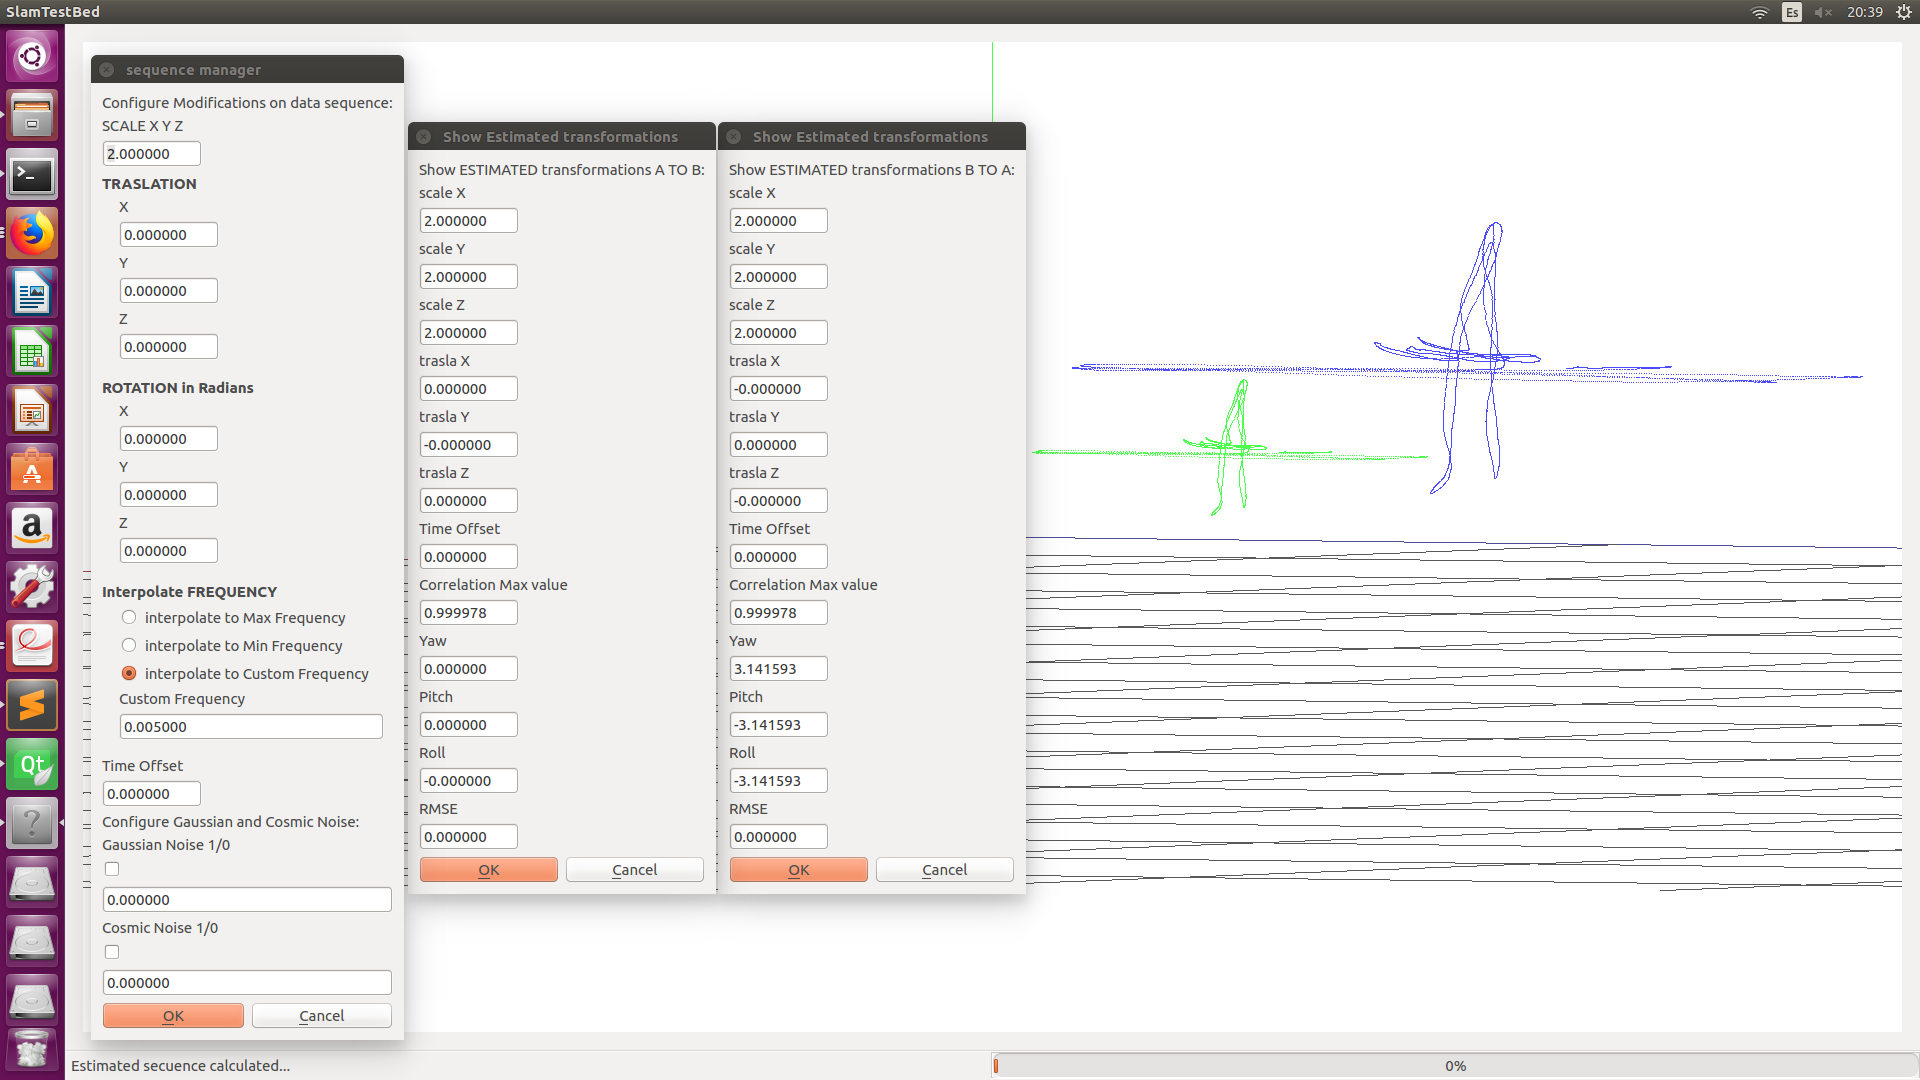
\includegraphics[height=10.0cm,width=15.0cm]{img/cap6/Escala_abba.png}}
\hspace{0.5cm}

\end{center}

\caption{Gráfico que muestra los resultados de la estimación tras una transformación de un cambio de escala.}
\end{figure}

El gráfico superior muestra los resultados de la estimación tras una transformación de un cambio de escala. Se aprecia en la captura de pantalla, como el dataset transformado es más grande que el dataset original. Como se puede observar el RMSE es 0.0 y el valor de la escala estimada coincide con el valor de la transformación de escala, en este caso es 2.0

\begin{figure}[H]
\begin{center}
\subfigure[]{\label{fig:opciones de View}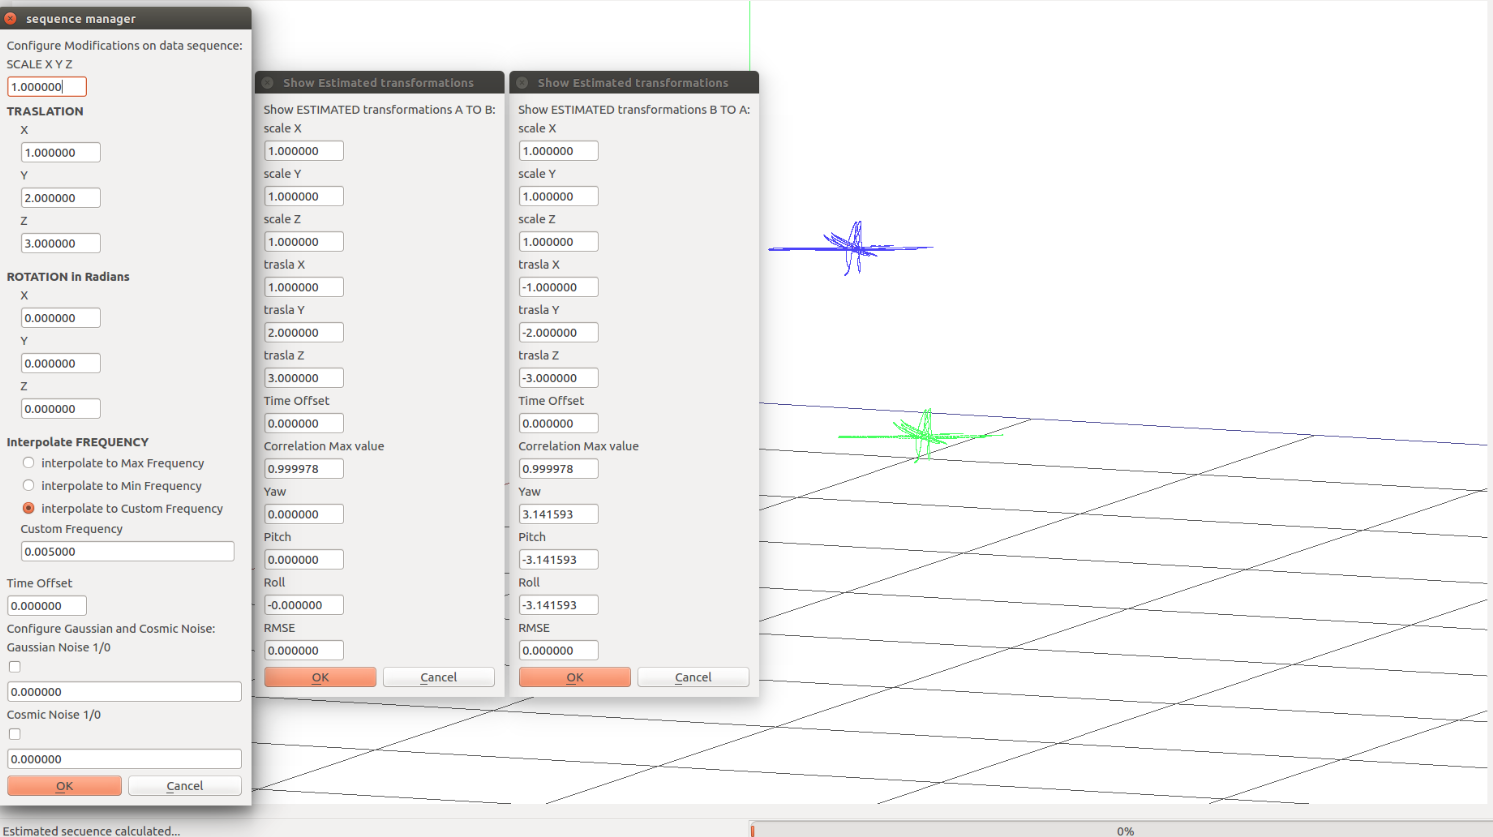
\includegraphics[height=10.0cm,width=15.0cm]{img/cap6/Traslation_abba.png}}
\hspace{0.5cm}

\end{center}

\caption{Gráfico que muestra los resultados de la estimación de un cambio de traslación.}
\end{figure}

La captura de pantalla superior muestra los resultados de la estimación tras realizar una traslación en el dataset original. Como puede observarse el RMSE es 0.0, y gráficamente el dataset transformado y estimado coinciden en cada posición 3D.  Es por este motivo por el que hay ausencia de puntos rojos en la representación 3D. Hay que recordar que el dataset estimado se presenta con puntos rojos. Cuando la estimación no es buena , el dataset transformado y estimado no coincidirán y podremos ver en pantalla los puntos rojos , allí donde precisamente no coincidan dataset estimado. En cuanto a los valores de la traslación estimada puede verse que coinciden con la transformación realizada.

\begin{figure}[H]
\begin{center}
\subfigure[]{\label{fig:opciones de View}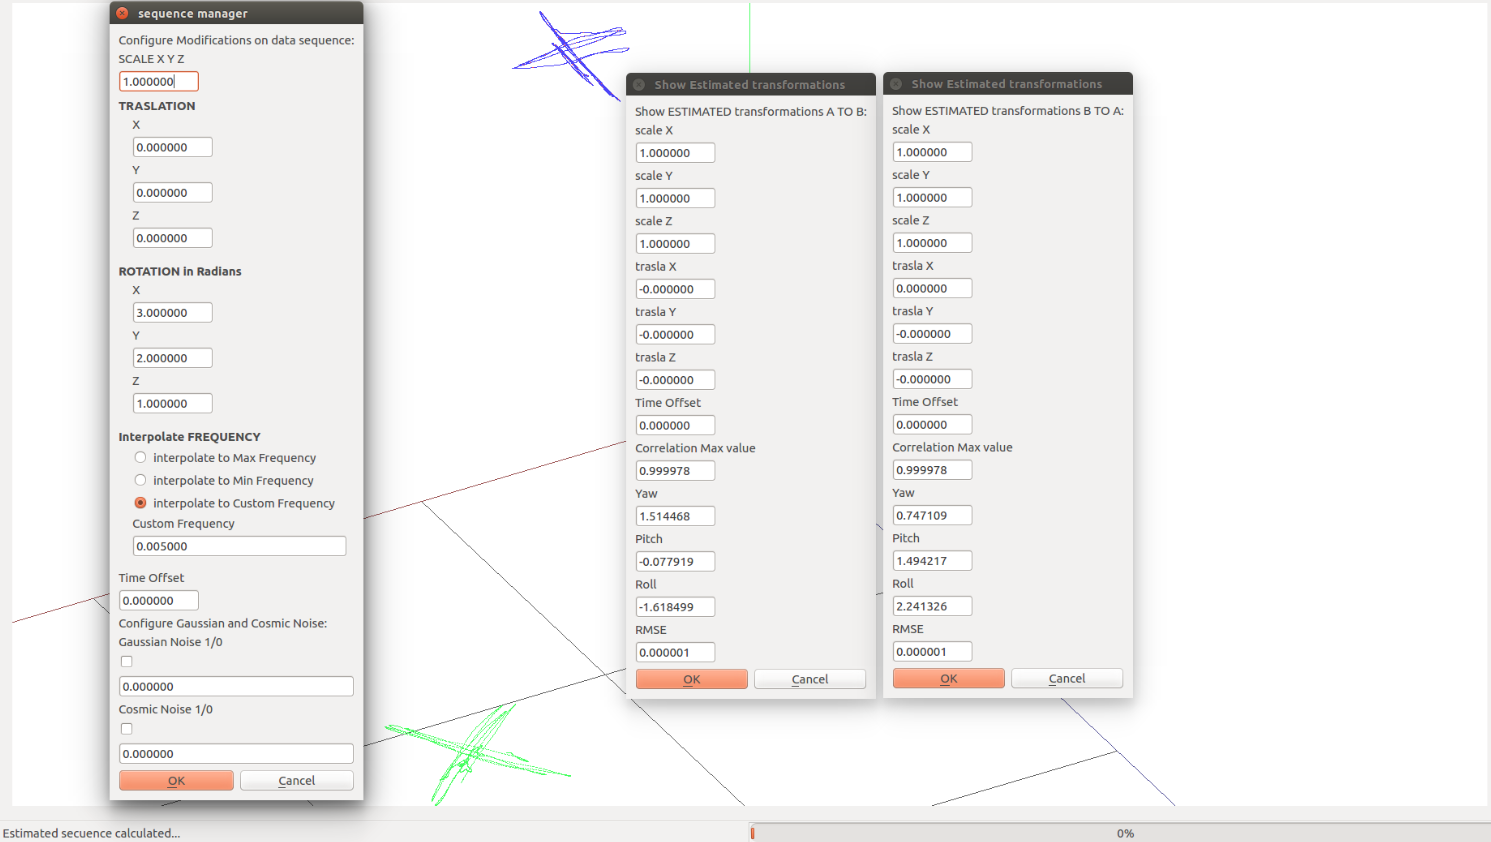
\includegraphics[height=10.0cm,width=15.0cm]{img/cap6/Rotation_abba.png}}
\hspace{0.5cm}

\end{center}

\caption{Gráfico que muestra los resultados de la estimación de un cambio de rotación.}
\end{figure}

En la captura de pantalla anterior, podremos observar el dataset original en verde, y el dataset transformado tras aplicar una rotación. La rotación se especifica en radianes. Como puede observarse, el error (RMSE) es mínimo 0.00001. Se puede comprobar que aunque la rotación realizada en los ejes X,Y,Z en la transformación ha sido respectivamente de 3.0, 2.0 y 1.0 radianes, en la estimación estos valores no coinciden, se ha aplicado otra rotación equivalente en radianes.



\section{Pruebas de transformaciones en parejas}

\begin{figure}[H]
\begin{center}
\subfigure[]{\label{fig:opciones de View}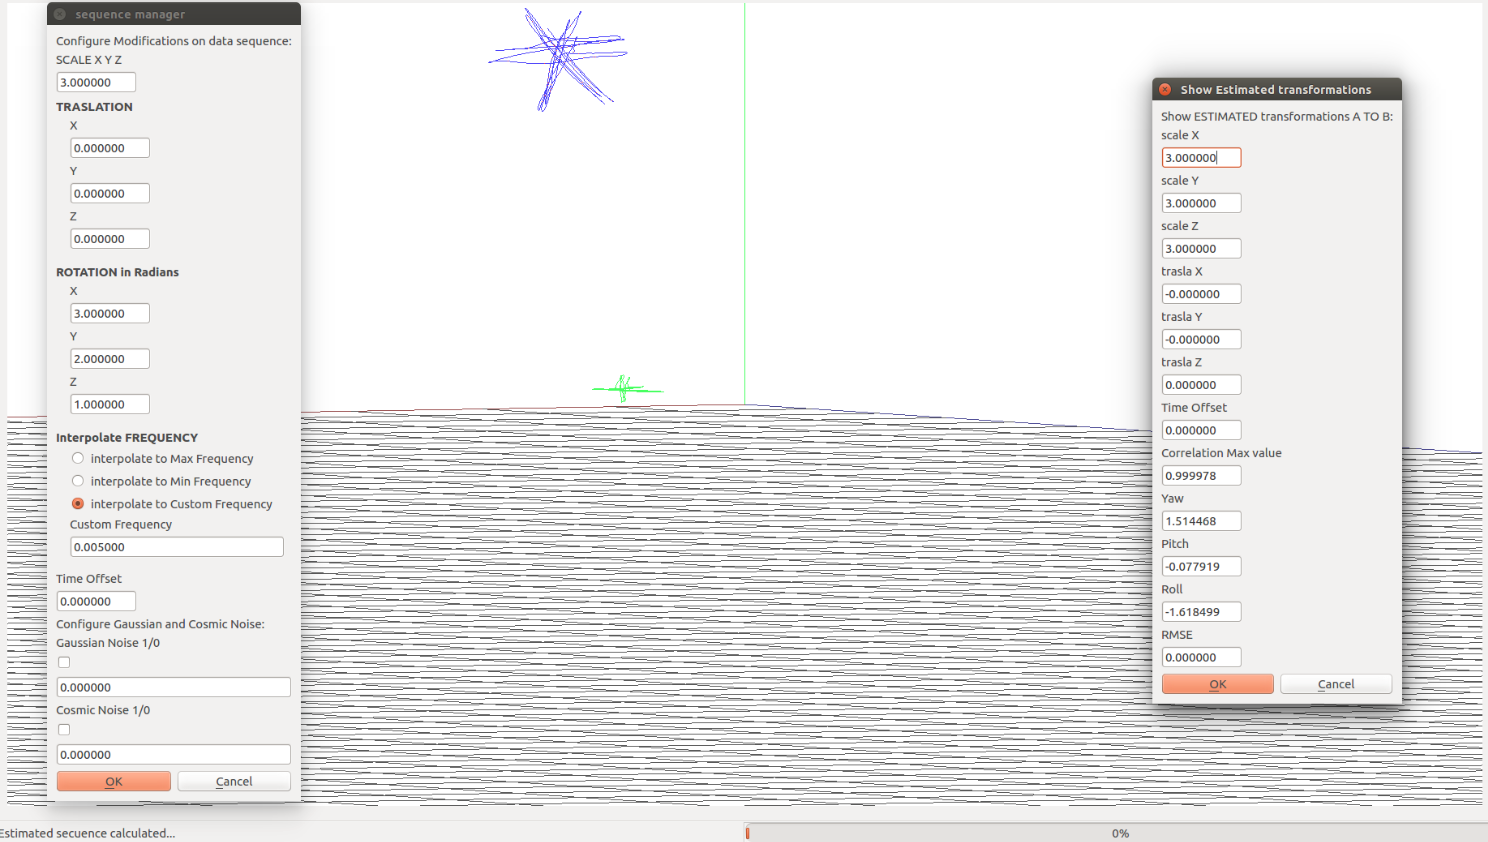
\includegraphics[height=10.0cm,width=15.0cm]{img/cap6/Escala_Traslacion.png}}
\hspace{0.5cm}

\end{center}

\caption{Gráfico que muestra los resultados de la estimación de un cambio de escala y traslación .}
\end{figure}

En la imagen superior, se muestra en color verde, el dataset groundtruth, y en azul el mismo dataset tras realizarle un par de transformaciones en escala y traslación.
En la ventana de la derecha se muestran los resultados de la transformación estimada, que coincide con la transformación realizada, además el RMSE es 0.
El dataset estimado , también se pinta en color rojo, pero en este caso la estimación es tan buena que coincide con el dataset transformado y no se aprecia ningún punto rojo.
En este caso la transformación realizada es de escala y traslación. Se puede comprobar que la estimación realizada es correcta ya que coinciden los valores de la escala y traslación estimados.



\begin{figure}[H]
\begin{center}
\subfigure[]{\label{fig:opciones de View}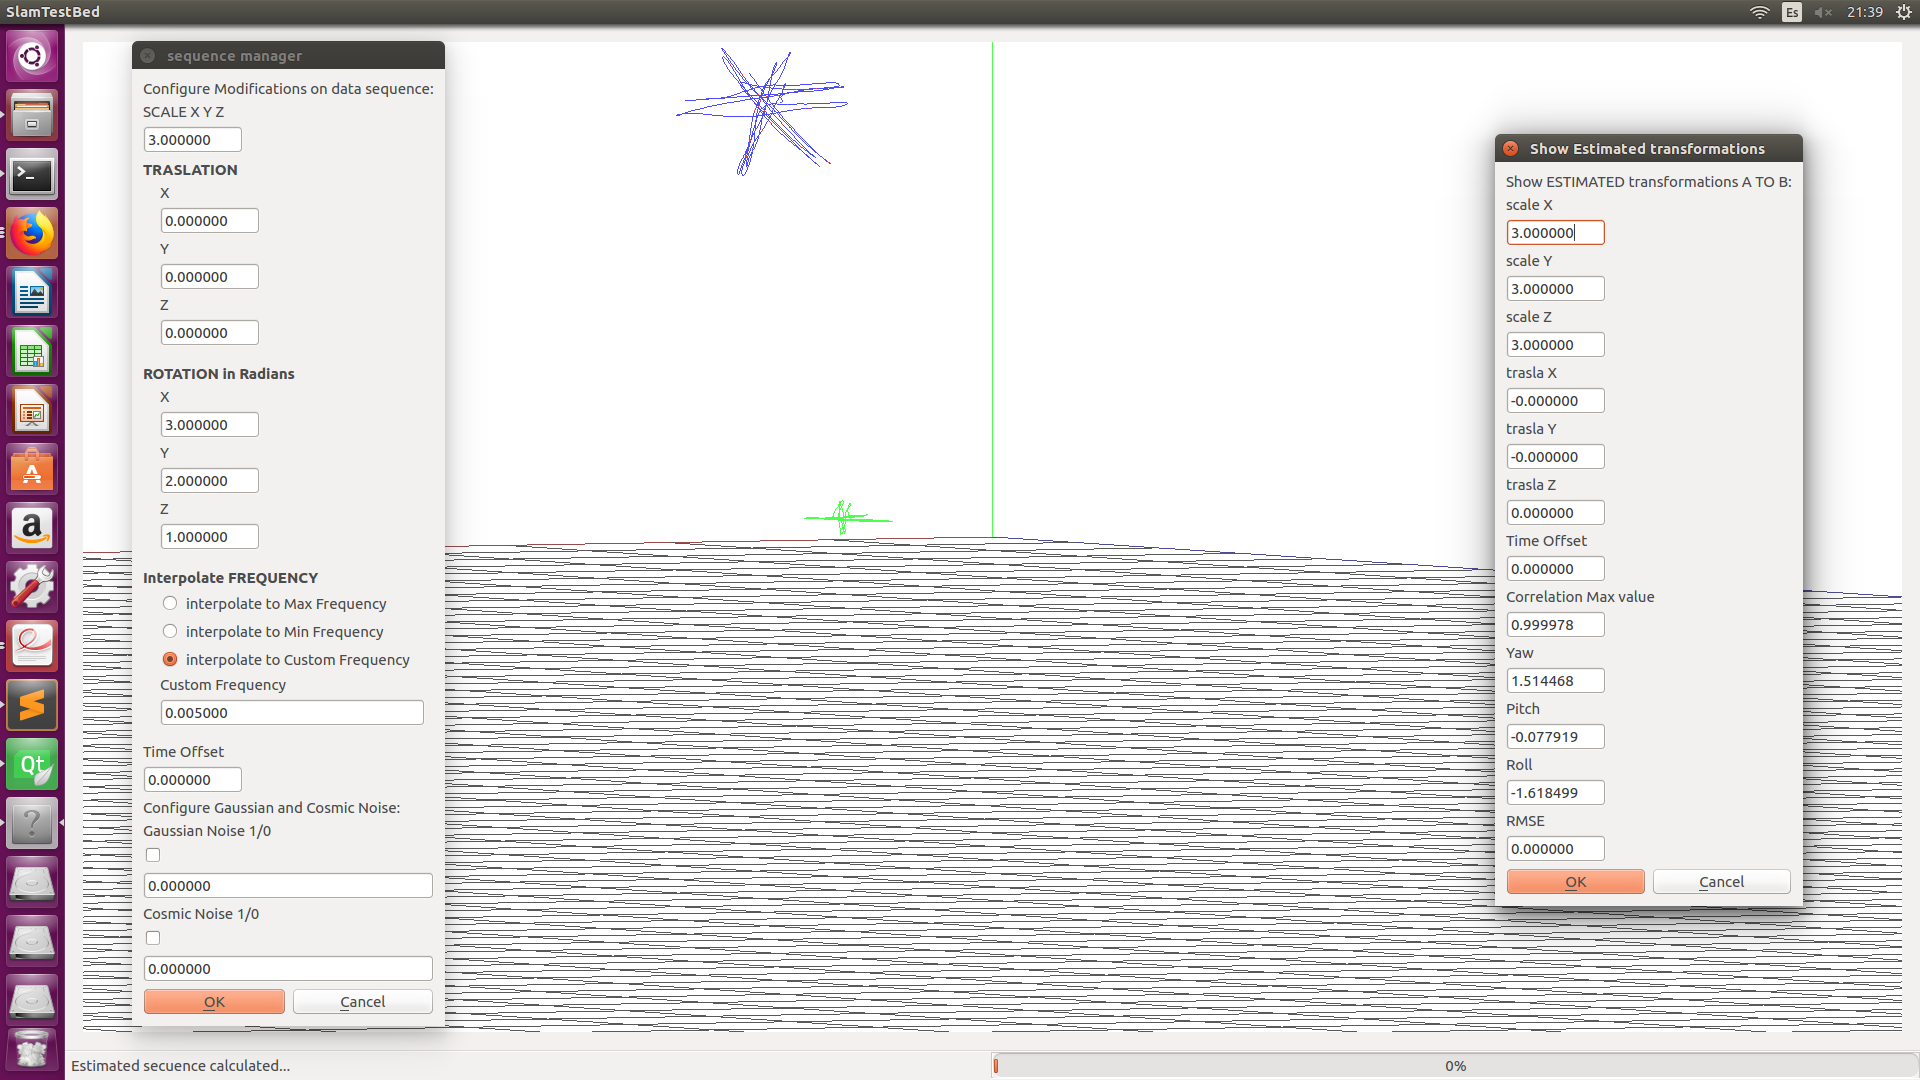
\includegraphics[height=10.0cm,width=15.0cm]{img/cap6/Escala_Rotation.png}}
\hspace{0.5cm}

\end{center}

\caption{Gráfico que muestra los resultados de la estimación de un cambio de escala y rotación.}
\end{figure}
En la imagen superior podemos ver los resultados de aplicar otras 2 transformaciones sobre el dataset original. En este caso se trata de una transformación en escala y rotación.
Tras realizar la estimación, el error medido entre el dataset estimado y el dataset transformado es 0.0 . Por tanto podemos decir que la estimación es exacta a la transformación realizada sobre el dataset original.

\begin{figure}[H]
\begin{center}
\subfigure[]{\label{fig:opciones de View}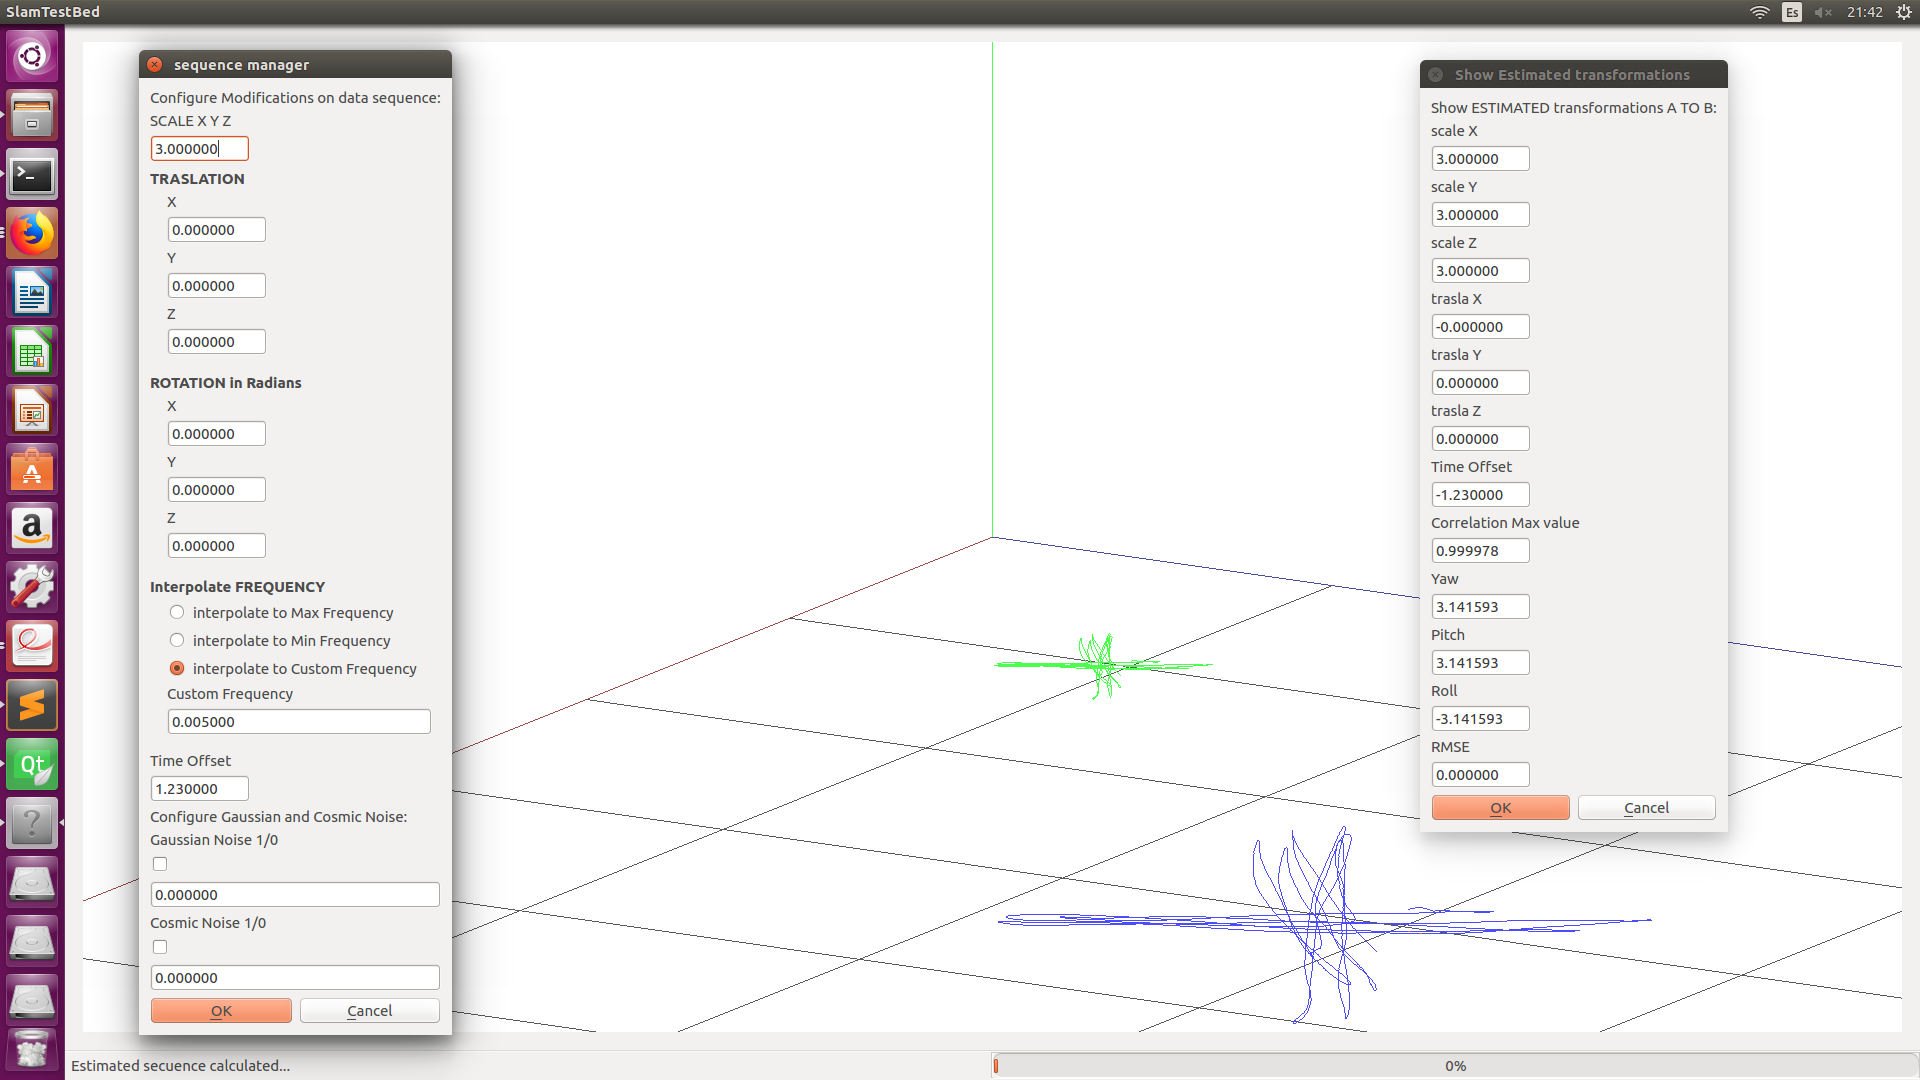
\includegraphics[height=10.0cm,width=15.0cm]{img/cap6/Escala_Offset.png}}
\hspace{0.5cm}

\end{center}

\caption{Gráfico que muestra los resultados de la estimación de un cambio de escala y offset.}
\end{figure}

En este caso, al dataset original (color verde) se le ha aplicado un par de transformaciones ( en escala y con offset), dando lugar al conjunto azul. En este caso tambien la estimación es buena , ya que el error RMSE da como resultado 0.0 y el cálculo del offset tambien coincide con el valor del offset que se ha aplicado en la transformación, salvo con signo negativo.


\begin{figure}[H]
\begin{center}
\subfigure[]{\label{fig:opciones de View}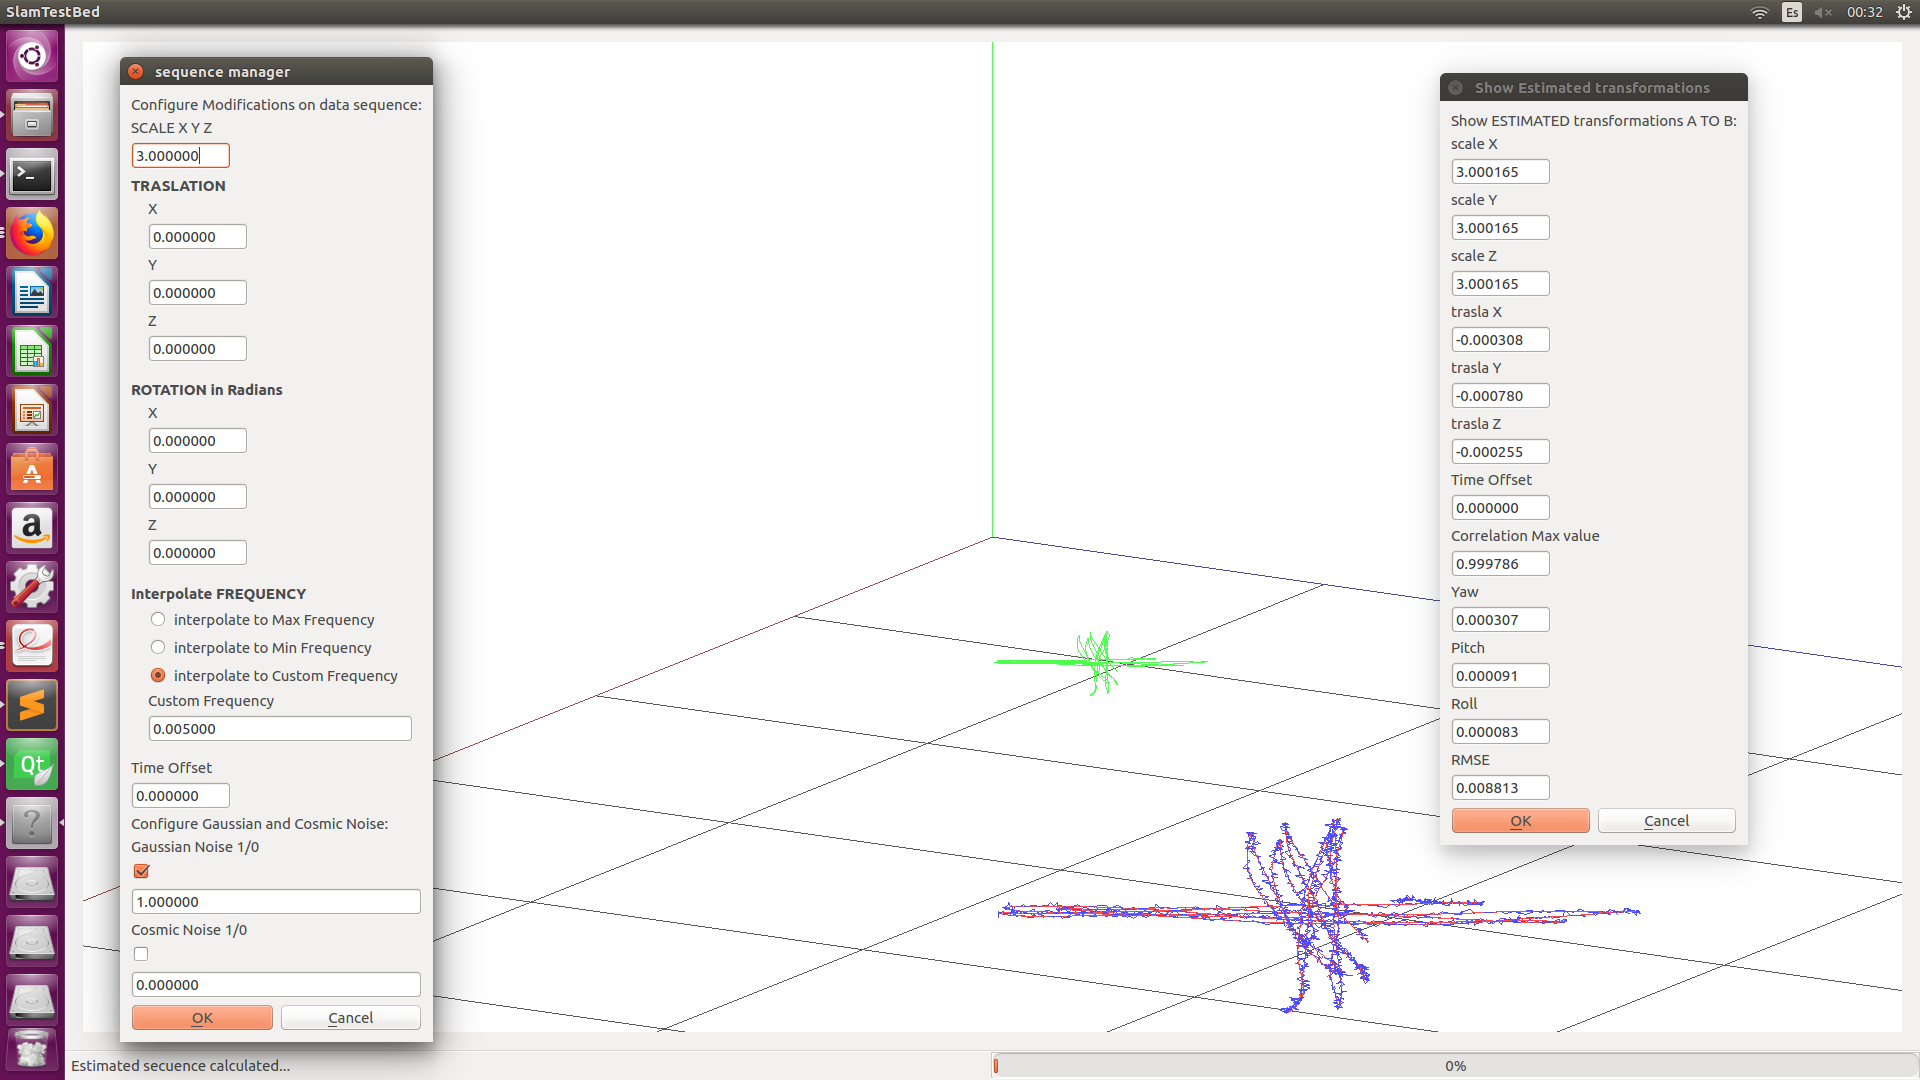
\includegraphics[height=10.0cm,width=15.0cm]{img/cap6/Escala_GaussNoise.png}}
\hspace{0.5cm}

\end{center}

\caption{Gráfico que muestra los resultados de la estimación de un cambio de escala y ruido Gaussiano .}
\end{figure}

En la imagen superior, se ha aplicado sobre el dataset original un cambio de escala y además se le ha añadido ruido Gaussiano, como puede verse en el dataset resultante (color azul). Las estimaciones obtenidas son buenas, pero el error RMSE calculado entre el dataset transformado y el dataset estimando ya no es 0.0, sino 0.008. Esta falta de precisión puede apreciarse a simple vista, ya que como el dataset estimado carece de ruido gaussiano, los puntos del dataset estimado no coinciden con los puntos del dataset transformado, y por tanto ahora si podemos ver buena parte de los puntos del dataset estimado (colo rojo).

\begin{figure}[H]
\begin{center}
\subfigure[]{\label{fig:opciones de View}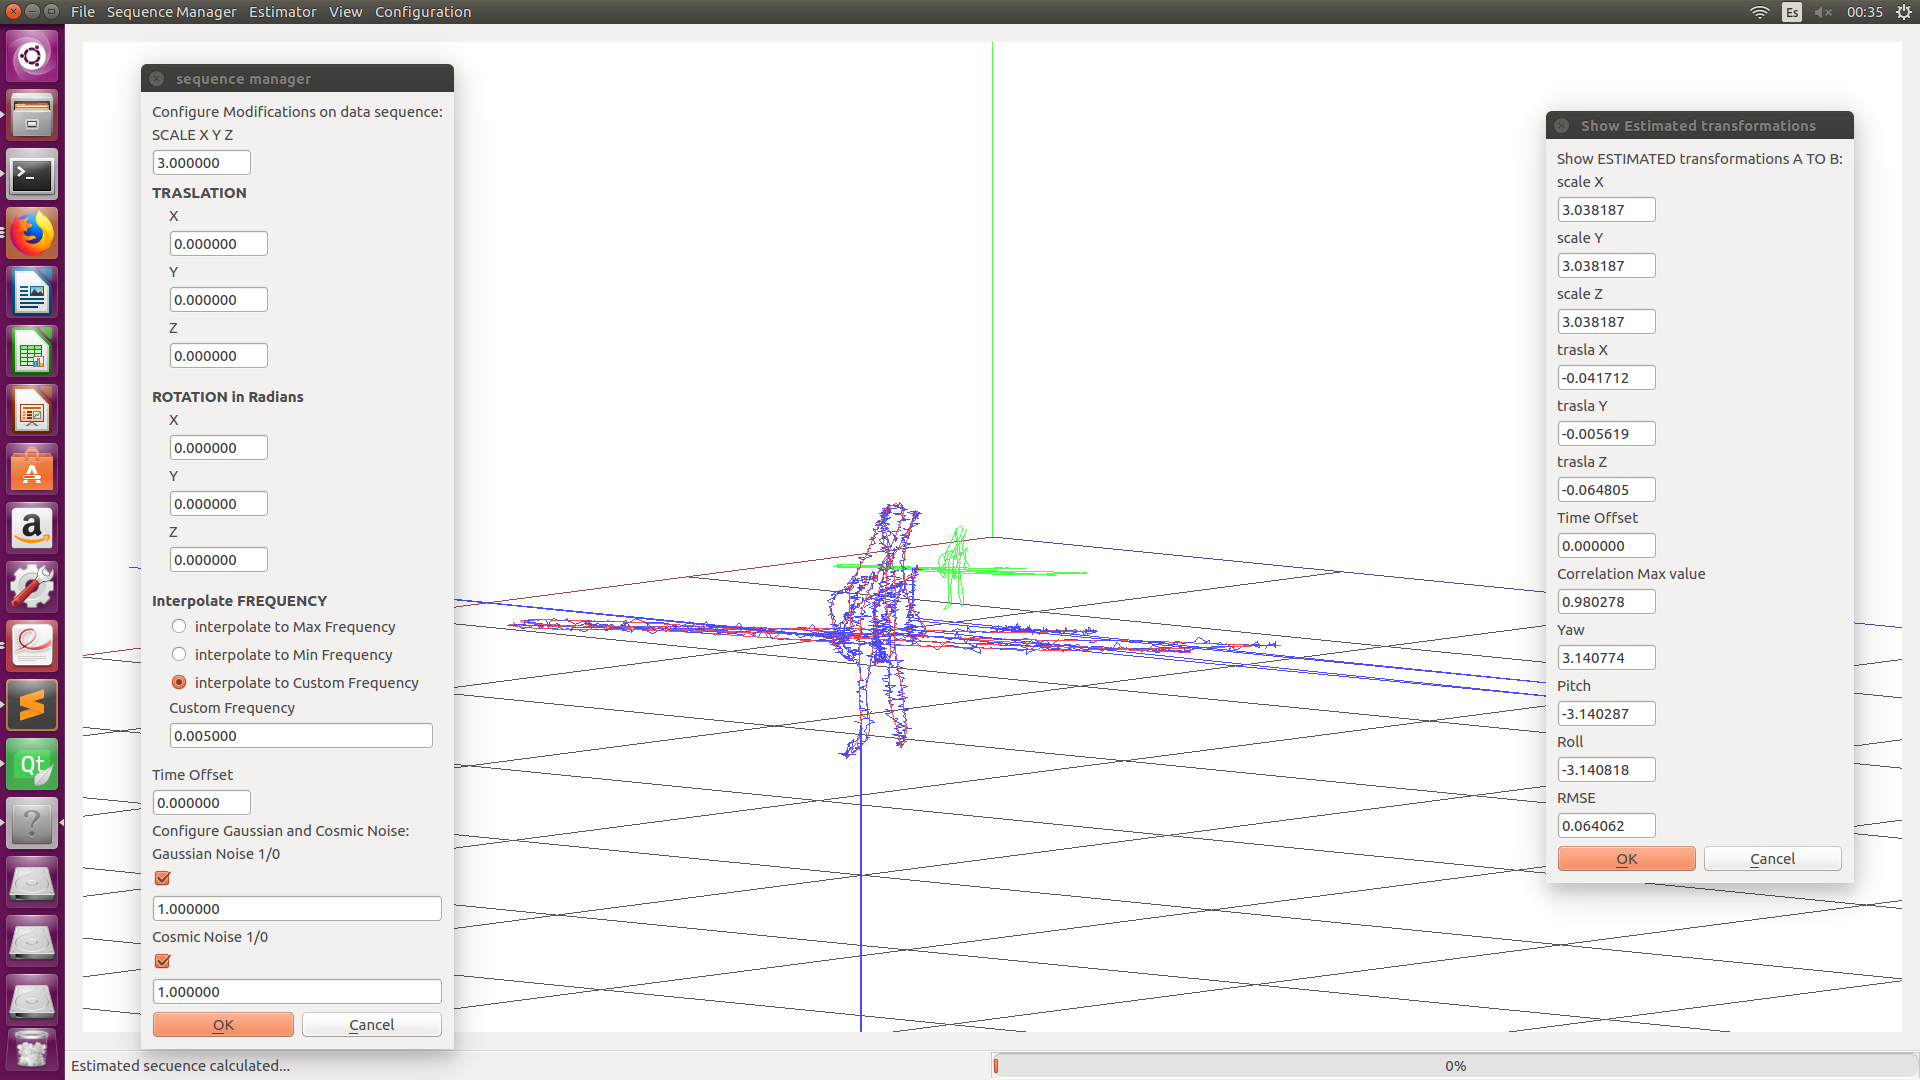
\includegraphics[height=10.0cm,width=15.0cm]{img/cap6/Escala_GaussCosmicNoise.png}}
\hspace{0.5cm}

\end{center}

\caption{Gráfico que muestra los resultados de la estimación de un cambio de escala y traslación .}
\end{figure}

En este caso, se ha aplicado sobre el dataset original un cambio de escala más ruido gaussiano y cósmico. Al tener ahora ruido cósmico, en algunos puntos del dataset transformado aparecen unos valores muy superiores a la media, estos valores desorbitados harán que aumente notablemente el error entre el dataset transformado y el dataset estimado. Para esta experimento , el valor RMSE es de 0.06. Aunque puede observarse que aún así, la posición de los puntos del dataset estimado coincide con la posición de los puntos del dataset transformado.

\begin{figure}[H]
\begin{center}
\subfigure[]{\label{fig:opciones de View}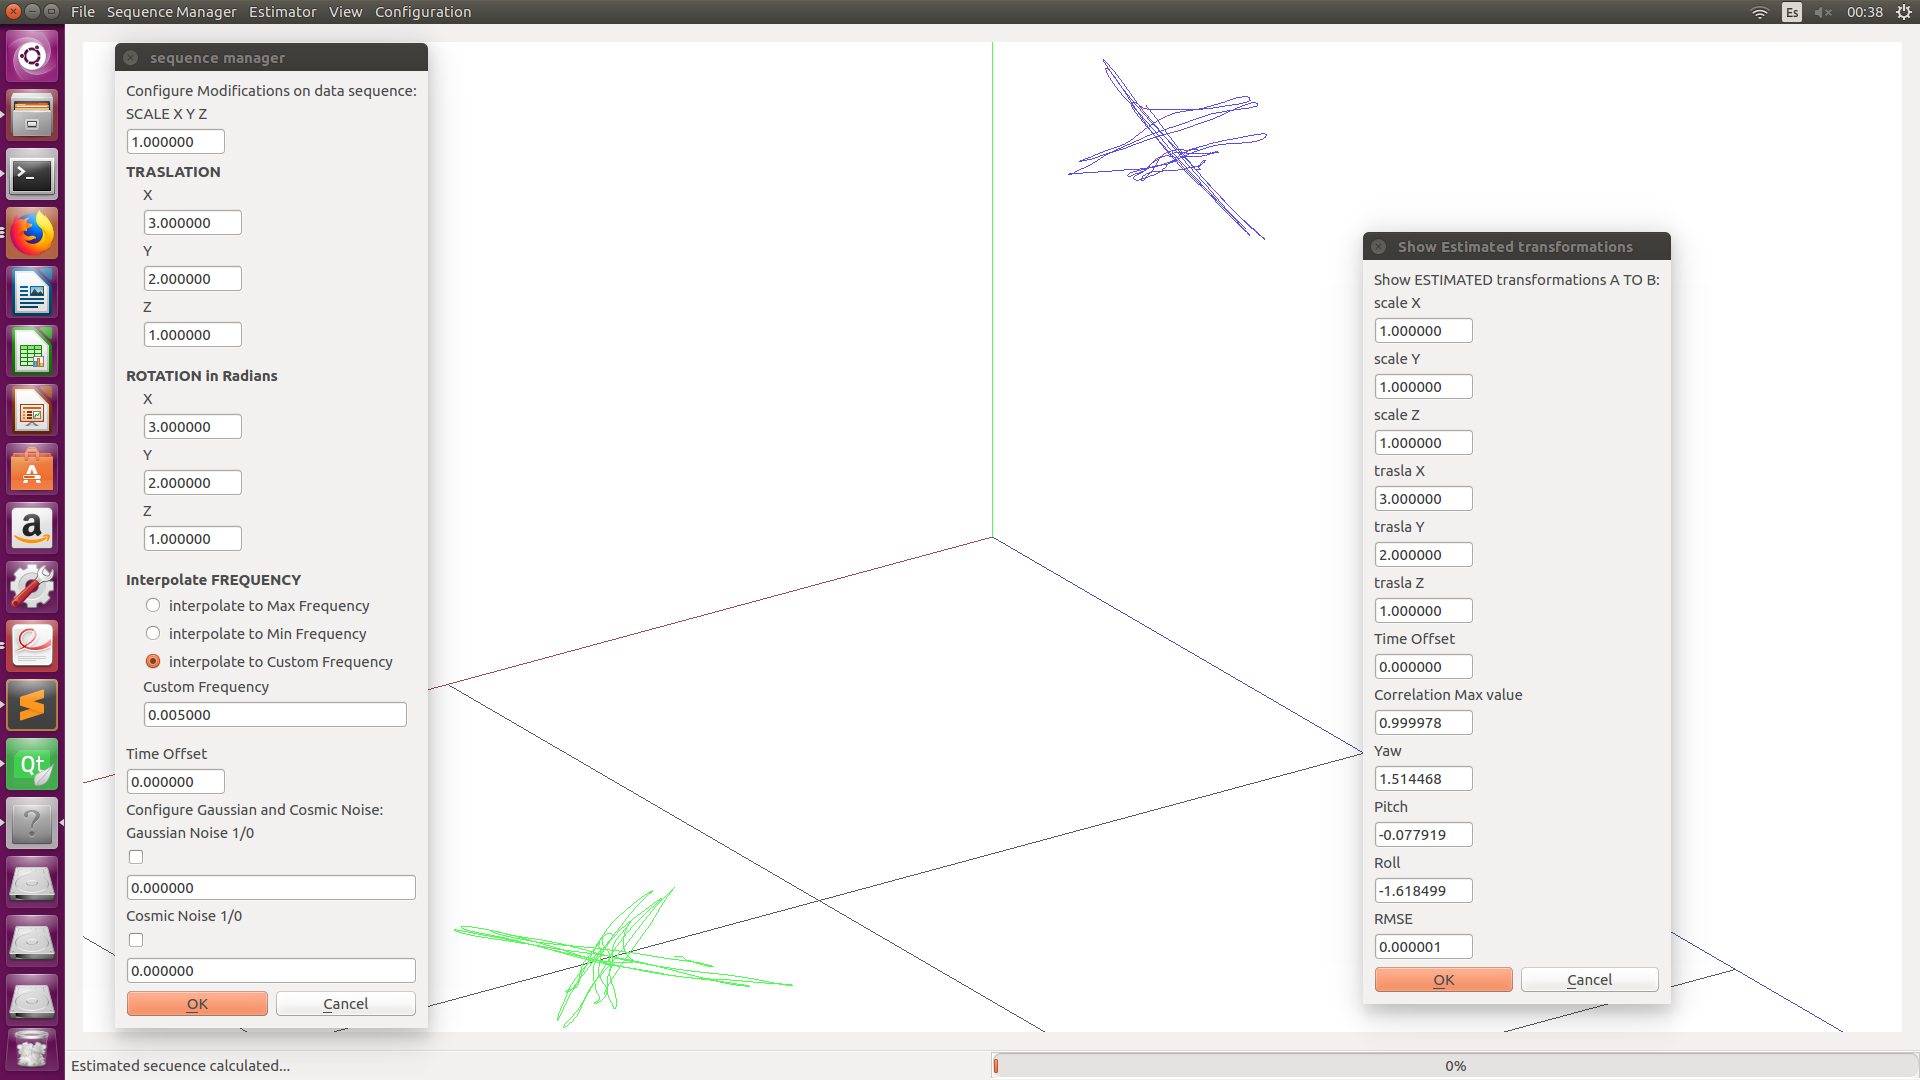
\includegraphics[height=10.0cm,width=15.0cm]{img/cap6/Trasla_Rota.png}}
\hspace{0.5cm}

\end{center}

\caption{Gráfico que muestra los resultados de la estimación de un cambio de traslación y rotación .}
\end{figure}

En este test, se han aplicado 2 transformaciones sobre el dataset original, una traslación y una rotación.
La estimación de la traslación y la rotación coinciden con los valores de las transformaciones. El error calculado entre el dataset estimado y el dataset transformado es 0.000001.
Podríamos considerarlo como 0.0


\begin{figure}[H]
\begin{center}
\subfigure[]{\label{fig:opciones de View}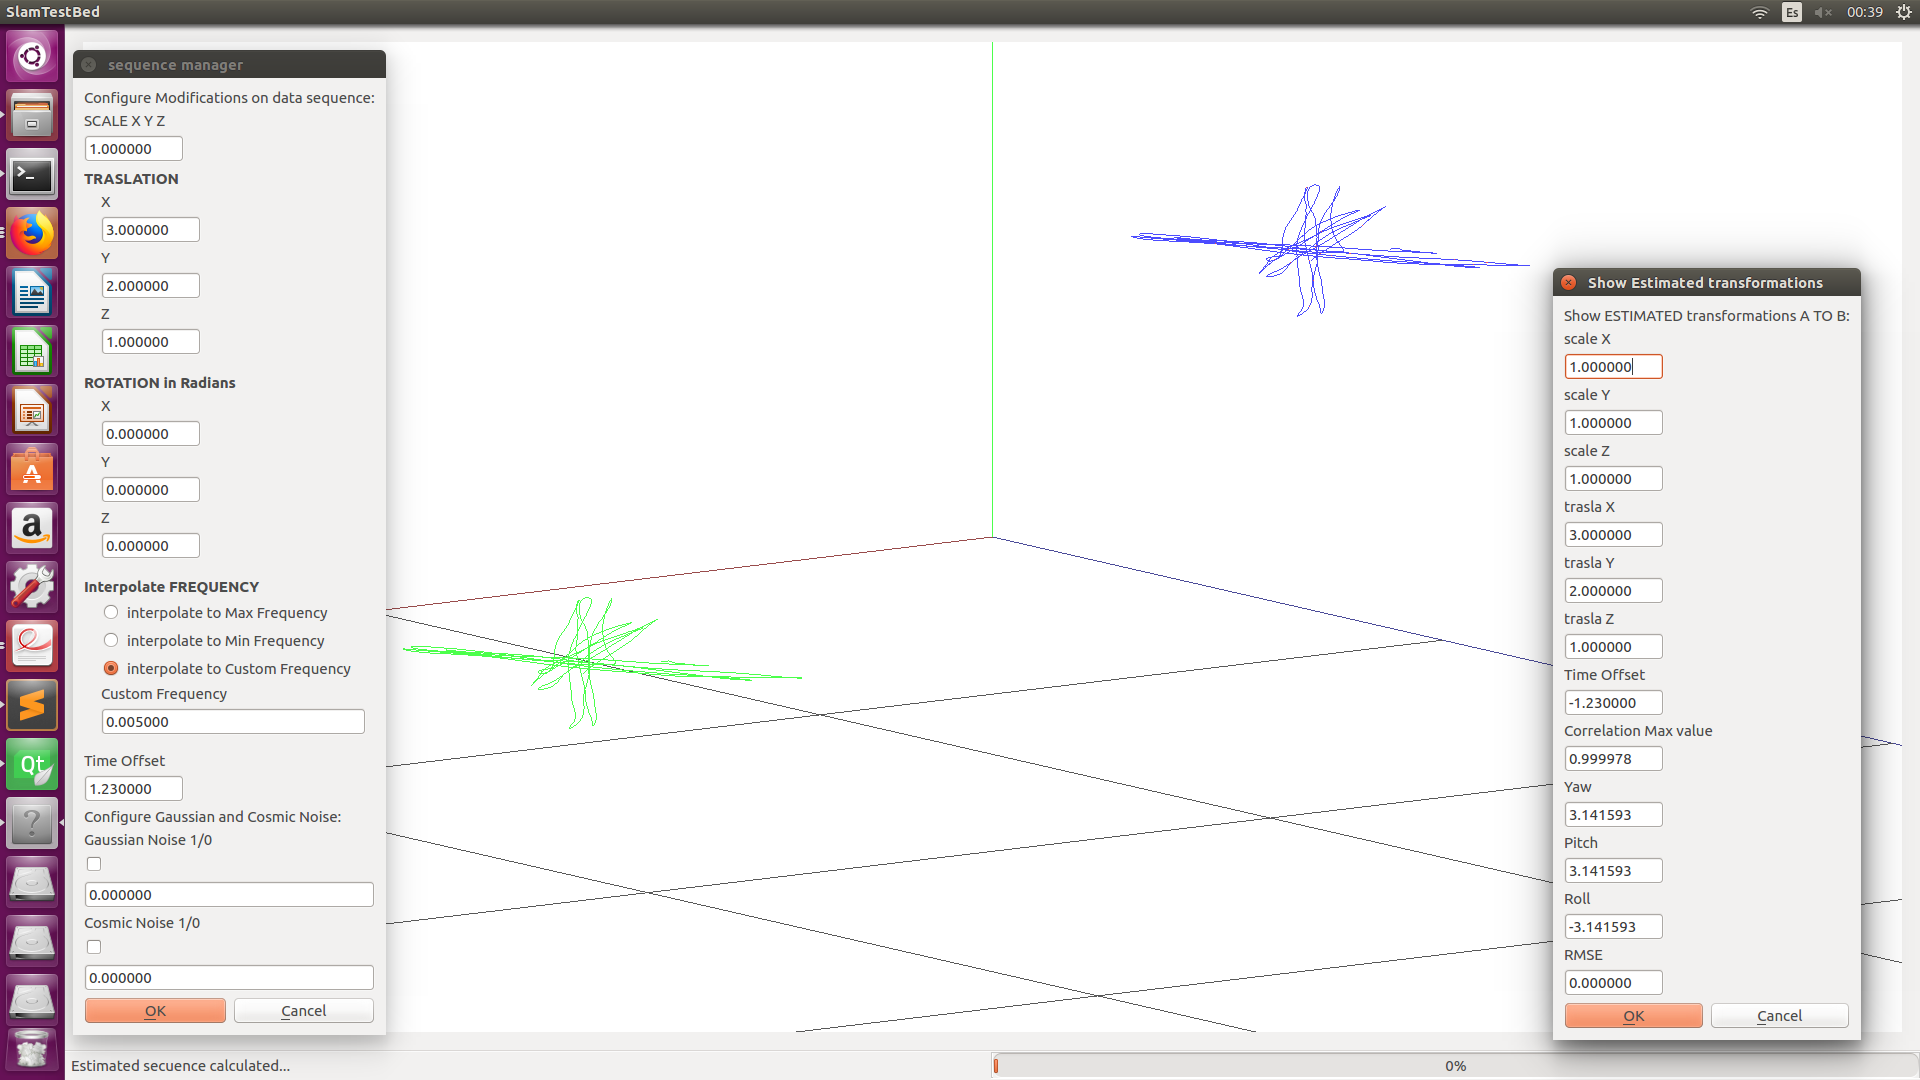
\includegraphics[height=10.0cm,width=15.0cm]{img/cap6/Trasla_Offset.png}}
\hspace{0.5cm}

\end{center}

\caption{Gráfico que muestra los resultados de la estimación de un cambio de traslación y offset .}
\end{figure}
En este caso, al dataset original (color verde) se le ha aplicado un par de transformaciones ( en traslación y con offset), dando lugar al dataset transformado (conjunto de puntos de color azul). En este caso tambien la estimación es buena , ya que el error RMSE da como resultado 0.0 y el cálculo del offset tambien coincide con el valor del offset que se ha aplicado en la transformación, salvo con signo negativo.


\begin{figure}[H]
\begin{center}
\subfigure[]{\label{fig:opciones de View}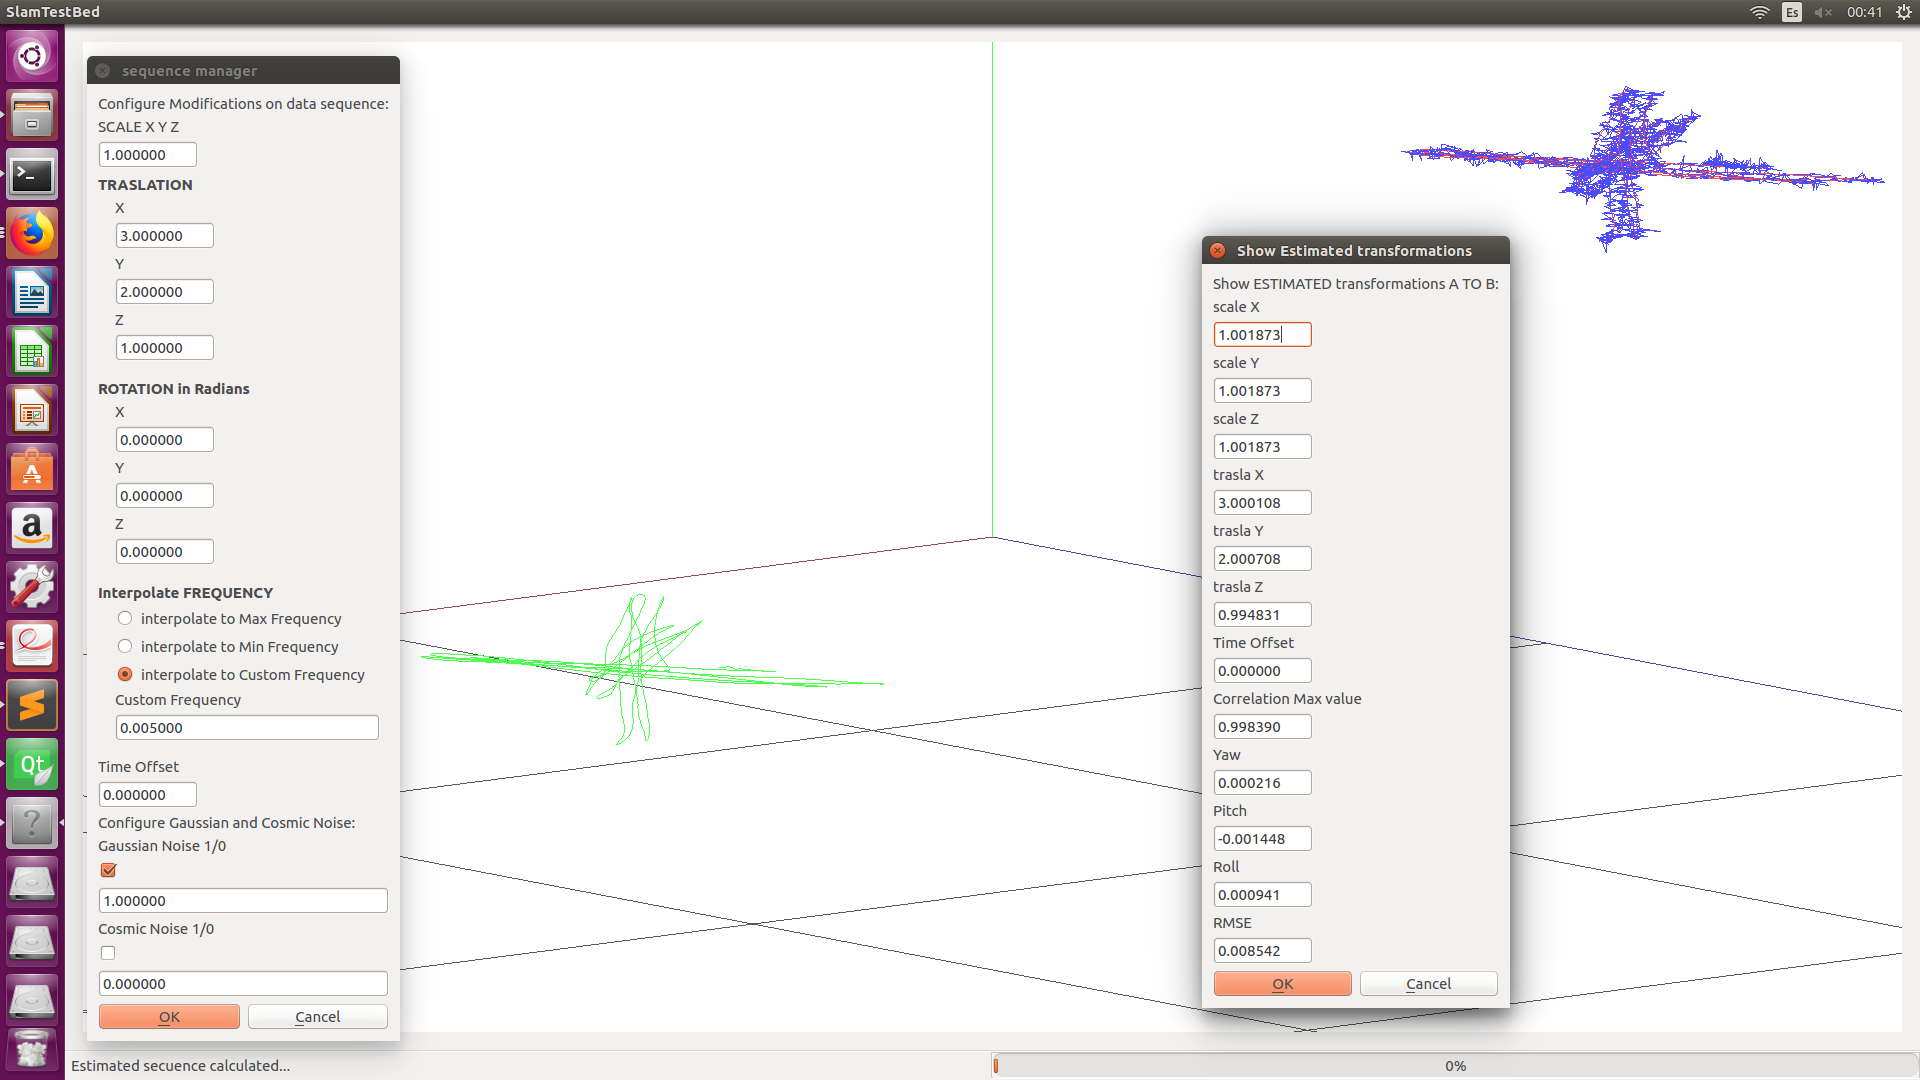
\includegraphics[height=10.0cm,width=15.0cm]{img/cap6/Trasla_GaussNoise.png}}
\hspace{0.5cm}

\end{center}

\caption{Gráfico que muestra los resultados de la estimación de un cambio de traslación y ruido gaussiano.}
\end{figure}
En la imagen superior, se ha aplicado sobre el dataset original un cambio de traslación y además se le ha añadido ruido Gaussiano, como puede verse en el dataset resultante (color azul). Las estimaciones obtenidas son buenas, pero el error RMSE calculado entre el dataset transformado y el dataset estimando ya no es 0.0, sino 0.008. Esta falta de precisión puede apreciarse a simple vista en el interfaz gráfico, ya que como el dataset estimado carece de ruido gaussiano , los puntos del dataset estimado no coinciden con los puntos del dataset transformado, y por tanto ahora si podemos ver buena parte de los puntos del dataset estimado (colo rojo).


\begin{figure}[H]
\begin{center}
\subfigure[]{\label{fig:opciones de View}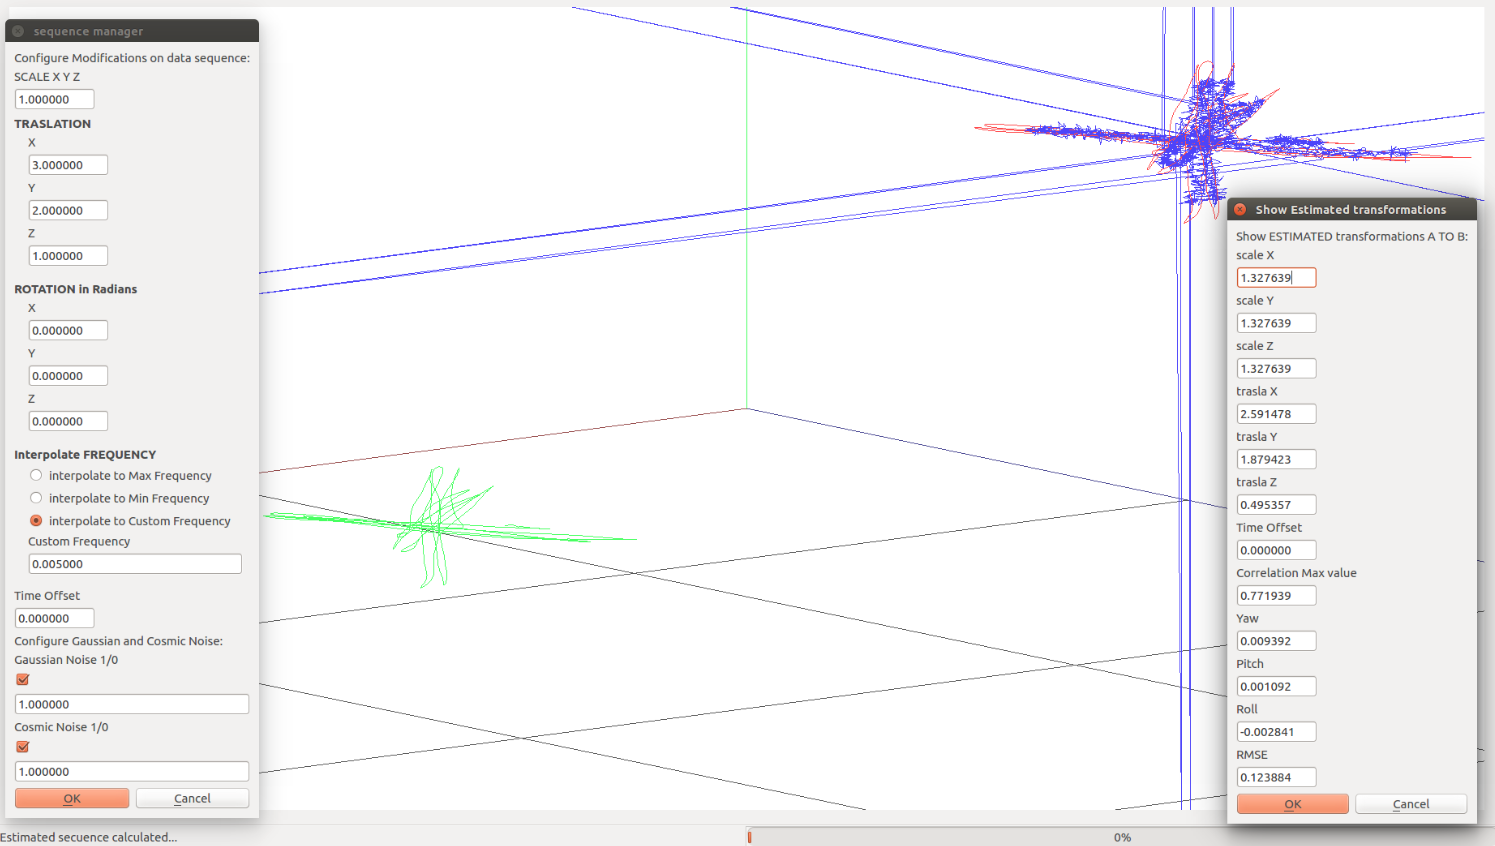
\includegraphics[height=10.0cm,width=15.0cm]{img/cap6/Trasla_GaussianCosmicNoise.png}}
\hspace{0.5cm}

\end{center}

\caption{Gráfico que muestra los resultados de la estimación de un cambio de traslación y ruido cósmico y gaussiano.}
\end{figure}
En este caso, se ha aplicado sobre el dataset original un cambio de traslación más ruido gaussiano y cósmico. Al tener ahora ruido cósmico, en algunos puntos del dataset transformado aparecen unos valores muy superiores al rango de valores del dataset , estos valores desorbitados harán que aumente notablemente el error entre el dataset transformado y el dataset estimado. Para esta experimento , el valor RMSE es de 0.12. Aunque puede observarse que aún así, la posición de los puntos del dataset estimado coincide con la posición de los puntos del dataset transformado.



\begin{figure}[H]
\begin{center}
\subfigure[]{\label{fig:opciones de View}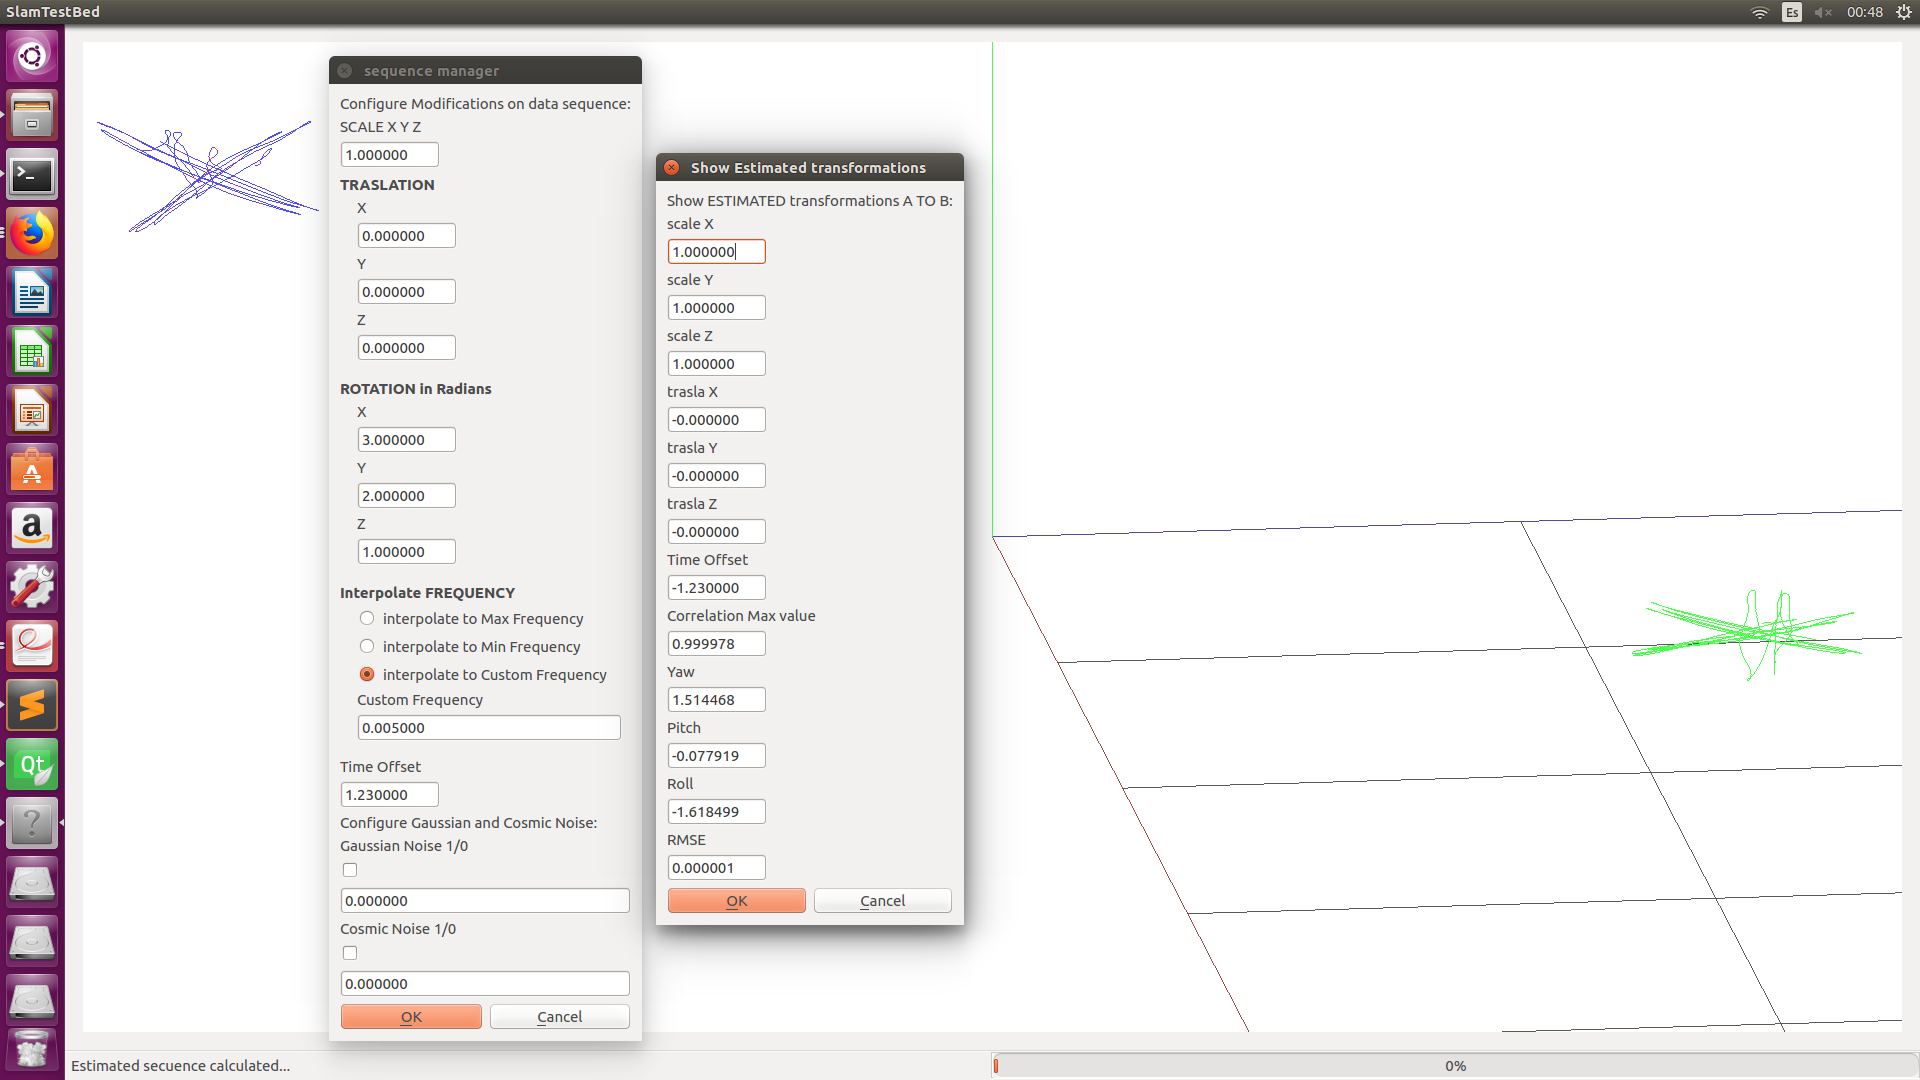
\includegraphics[height=10.0cm,width=15.0cm]{img/cap6/Rota_Offset.png}}
\hspace{0.5cm}

\end{center}

\caption{Gráfico que muestra los resultados de la estimación de un cambio de rotación y offset.}
\end{figure}

En este caso, al dataset original (color verde) se le ha aplicado un par de transformaciones ( en rotación y con offset tenmporal), dando lugar al dataset transformado (conjunto de puntos de color azul). En este caso tambien la estimación es buena , ya que el error RMSE da como resultado 0.0 y el cálculo del offset tambien coincide con el valor del offset que se ha aplicado en la transformación, salvo con signo negativo.



\begin{figure}[H]
\begin{center}
\subfigure[]{\label{fig:opciones de View}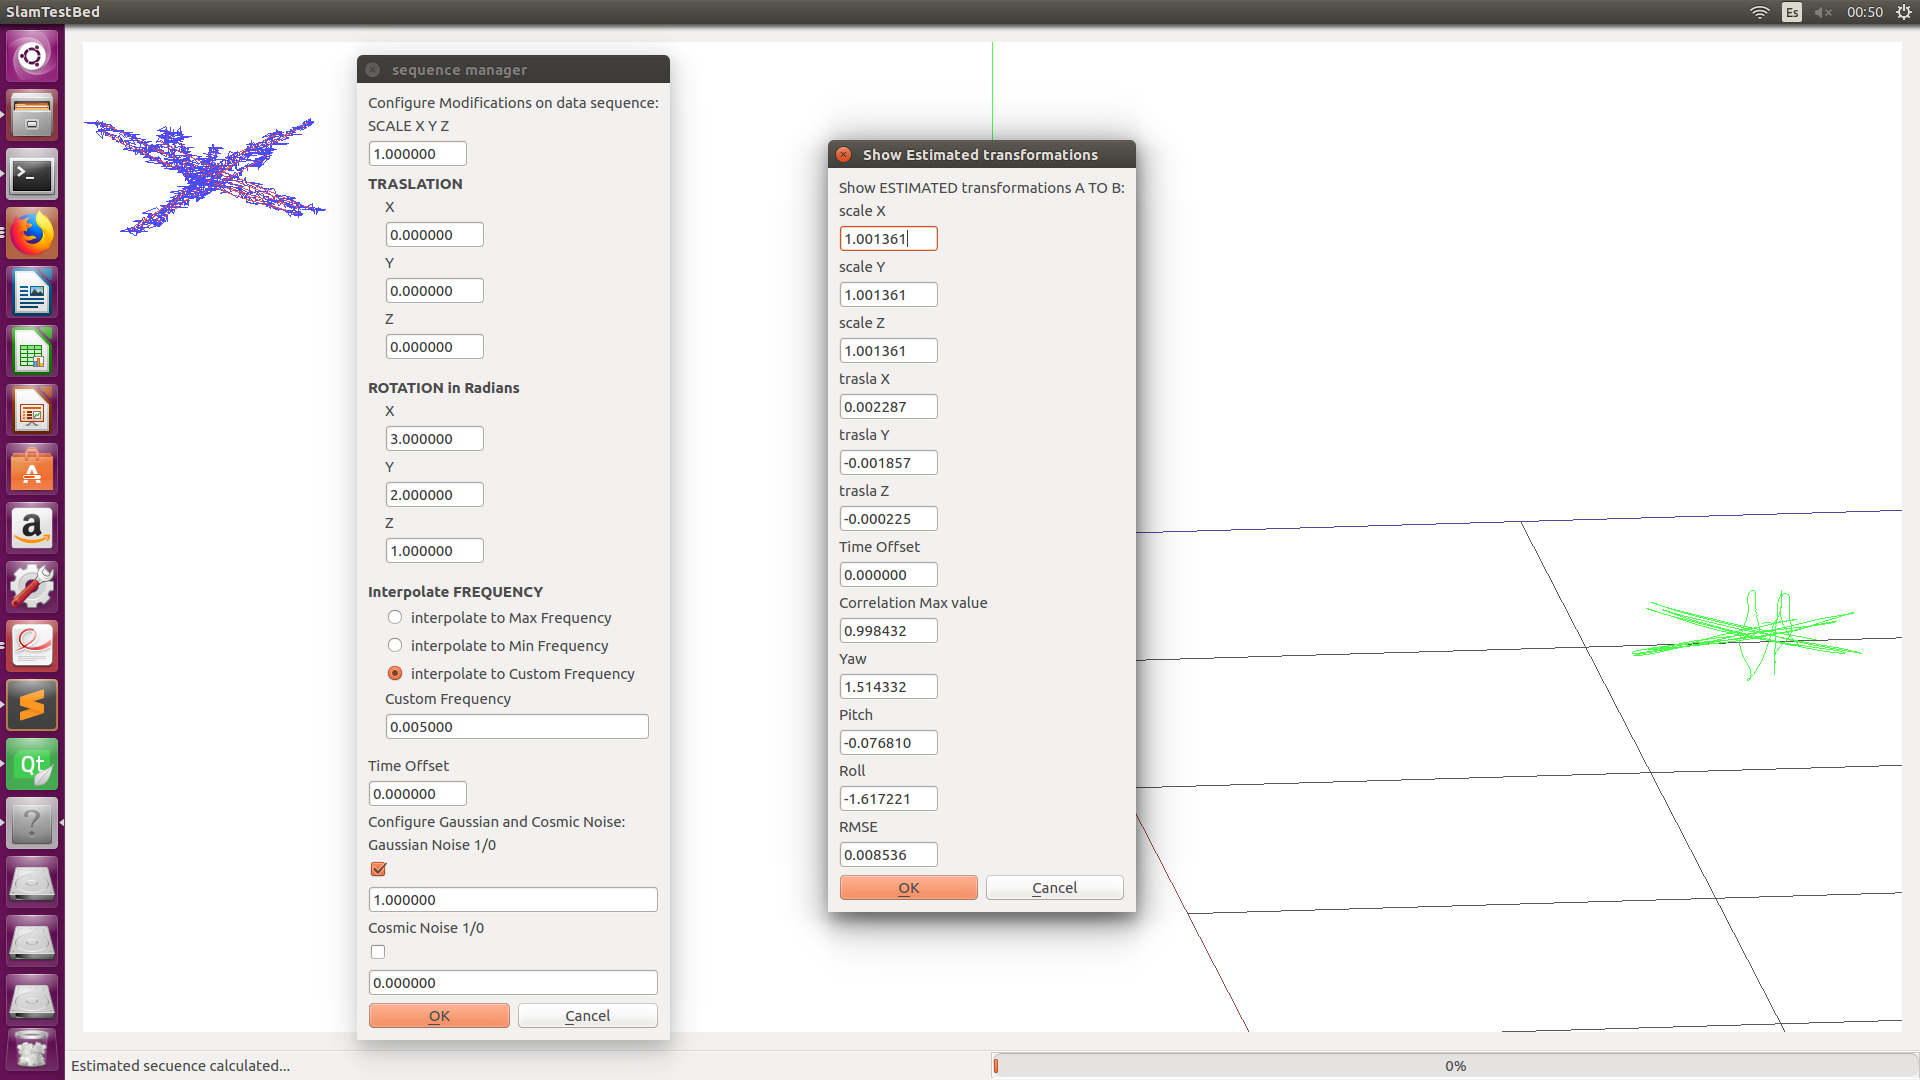
\includegraphics[height=10.0cm,width=15.0cm]{img/cap6/Rota_GaussNoise.png}}
\hspace{0.5cm}

\end{center}

\caption{Gráfico que muestra los resultados de la estimación de un cambio de rotación y ruido gaussiano.}
\end{figure}
En la imagen superior, se ha aplicado sobre el dataset original un cambio de rotación y además se le ha añadido ruido Gaussiano, como puede verse en el dataset resultante (color azul). Las estimaciones obtenidas son buenas, pero el error RMSE calculado entre el dataset transformado y el dataset estimado ya no es 0.0, sino 0.008. Esta falta de precisión puede apreciarse a simple vista en el interfaz gráfico, ya que como el dataset estimado carece de ruido gaussiano , los puntos del dataset estimado no coinciden con los puntos del dataset transformado, y por tanto ahora si podemos ver buena parte de los puntos del dataset estimado (colo rojo).




\begin{figure}[H]
\begin{center}
\subfigure[]{\label{fig:opciones de View}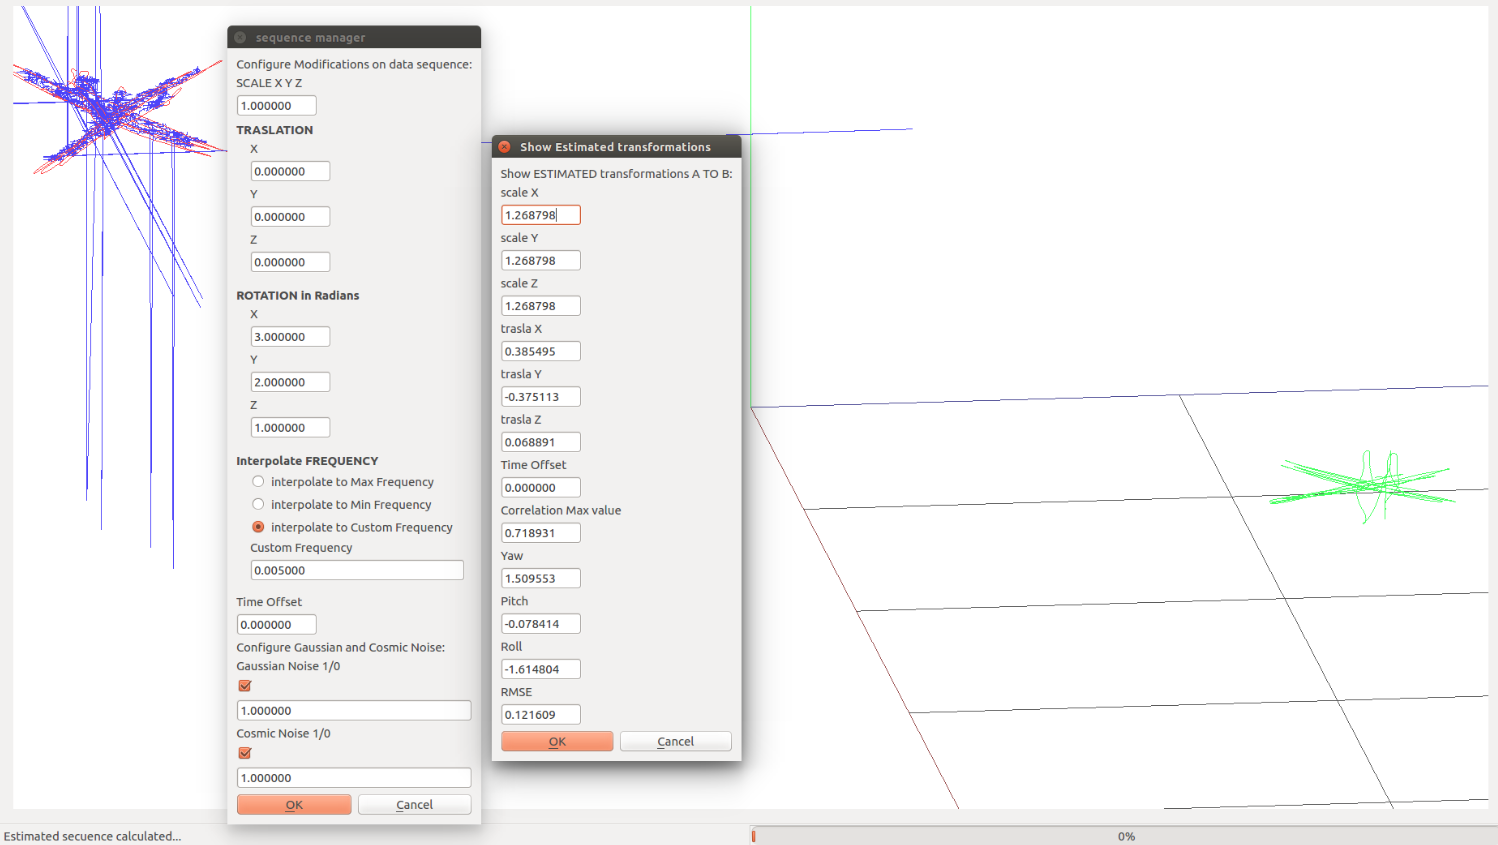
\includegraphics[height=10.0cm,width=15.0cm]{img/cap6/Rota_Gauss_Cosmic.png}}
\hspace{0.5cm}

\end{center}

\caption{Gráfico que muestra los resultados de la estimación de un cambio de rotación y ruido cósmico y gaussiano.}
\end{figure}

En este caso, se ha aplicado sobre el dataset original un cambio de rotación más ruido gaussiano y cósmico. Al tener ahora ruido cósmico, en algunos puntos del dataset transformado aparecen unos valores muy superiores al rango de valores del dataset , estos valores desorbitados harán que aumente notablemente el error entre el dataset transformado y el dataset estimado. Para esta experimento, el valor RMSE es de 0.12. Aunque puede observarse que aún así, la posición de los puntos del dataset estimado coincide con la posición de los puntos del dataset transformado.




\section{Pruebas de transformaciones combinadas}

En este apartado mostraremos los resultados de las estimaciones tras realizar varias transformaciones combinadas. En todas se utiliza la interpolación de tiempo a 0.005 segundos


\begin{figure}[H]
\begin{center}
\subfigure[]{\label{fig:opciones de View}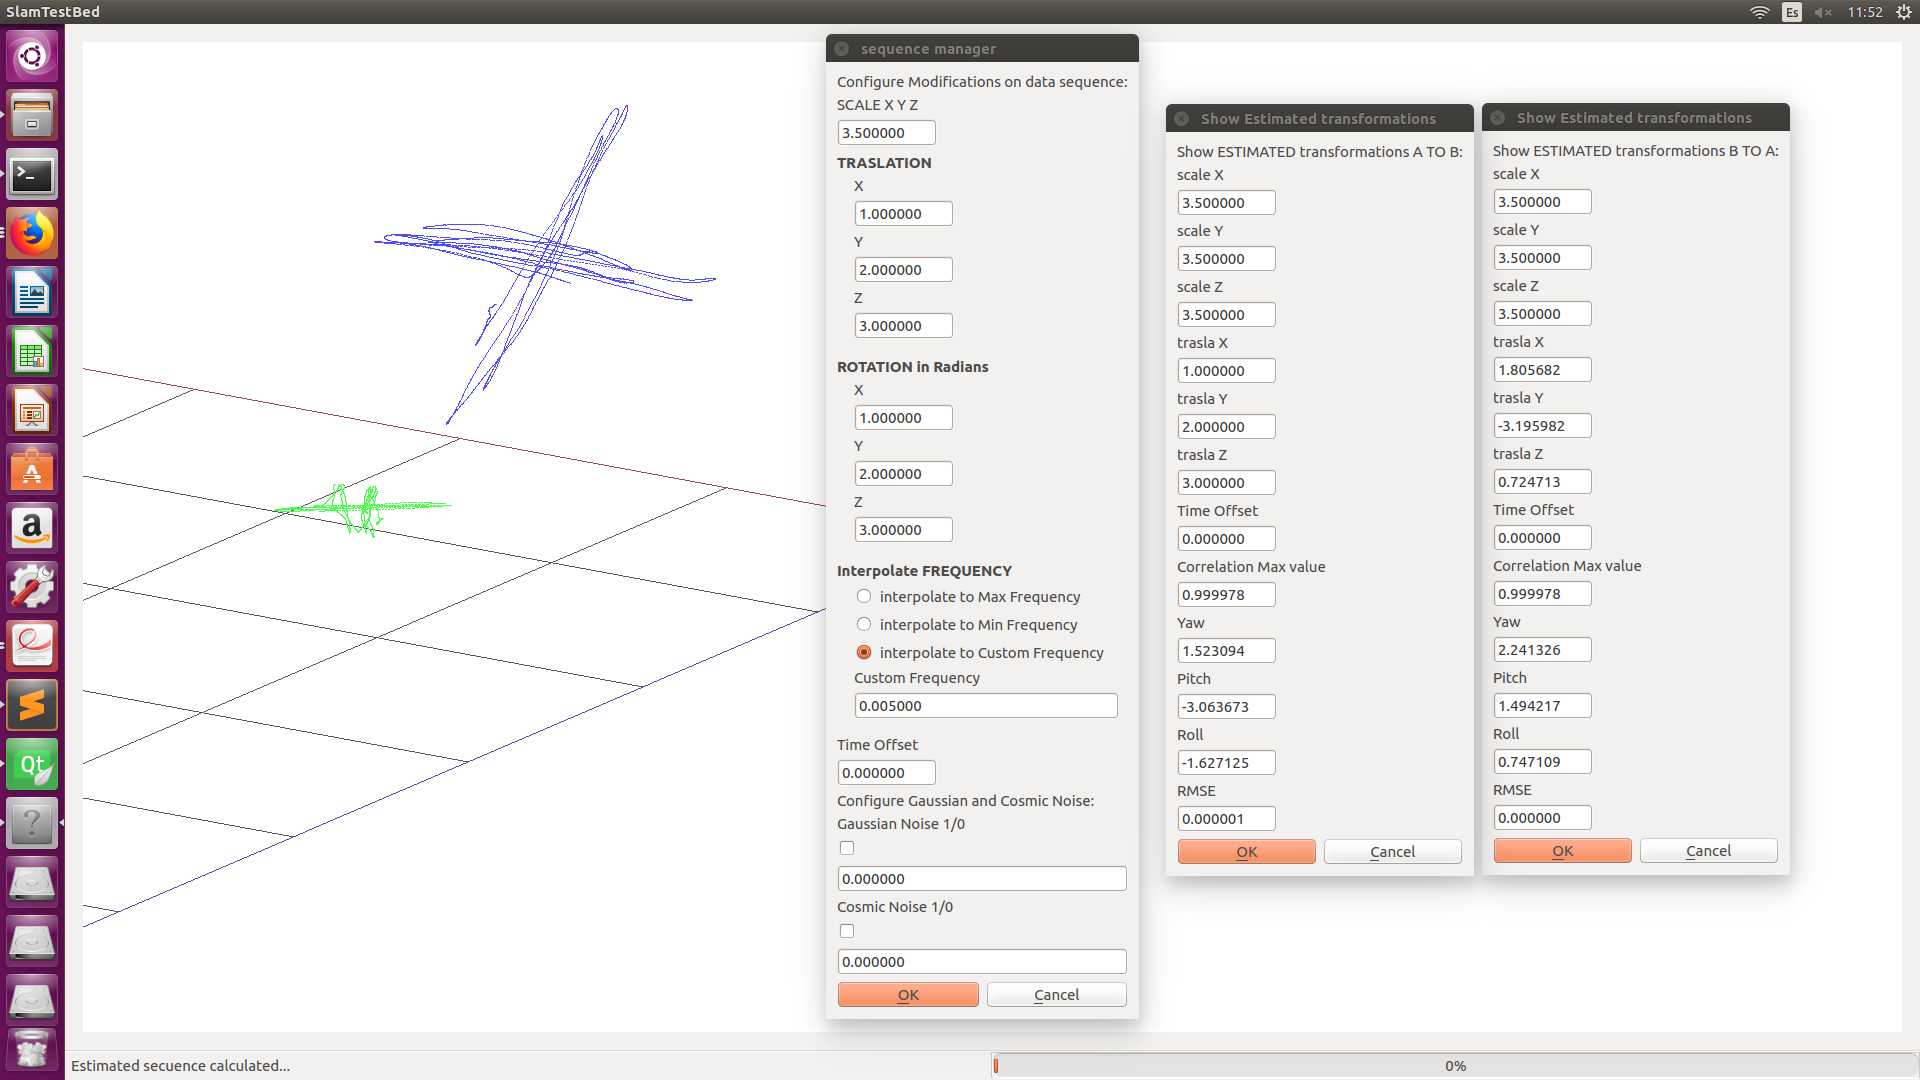
\includegraphics[height=10.0cm,width=15.0cm]{img/cap6/Escala_Trasla_Rota_abba.png}}
\hspace{0.5cm}

\end{center}

\caption{Gráfico que muestra los resultados de la estimación de un cambio de escala y traslación .}
\end{figure}

En la imagen superior se realiza la estimación de las transformaciones necesarias para pasar del datasetA al datasetB . En este caso se ha aplicado una transformación combinada de Escala, Traslación y Rotación. En verde puede verse el dataset original y en azul el dataset transformado, en rojo se aprecia el dataset estimado.
Se puede ver gráficamente como el dataset estimado se ajusta con gran precisión al dataset transformado (azul).
Por otra parte el RMSE entre el dataset transformado y el dataset estimado es de 0.0
Además las transformaciones se han calculado en los 2 sentidos, desde el dataSet A  al dataSet B y desde el dataSetB al dataSet A.


\begin{figure}[H]
\begin{center}
\subfigure[]{\label{fig:opciones de View}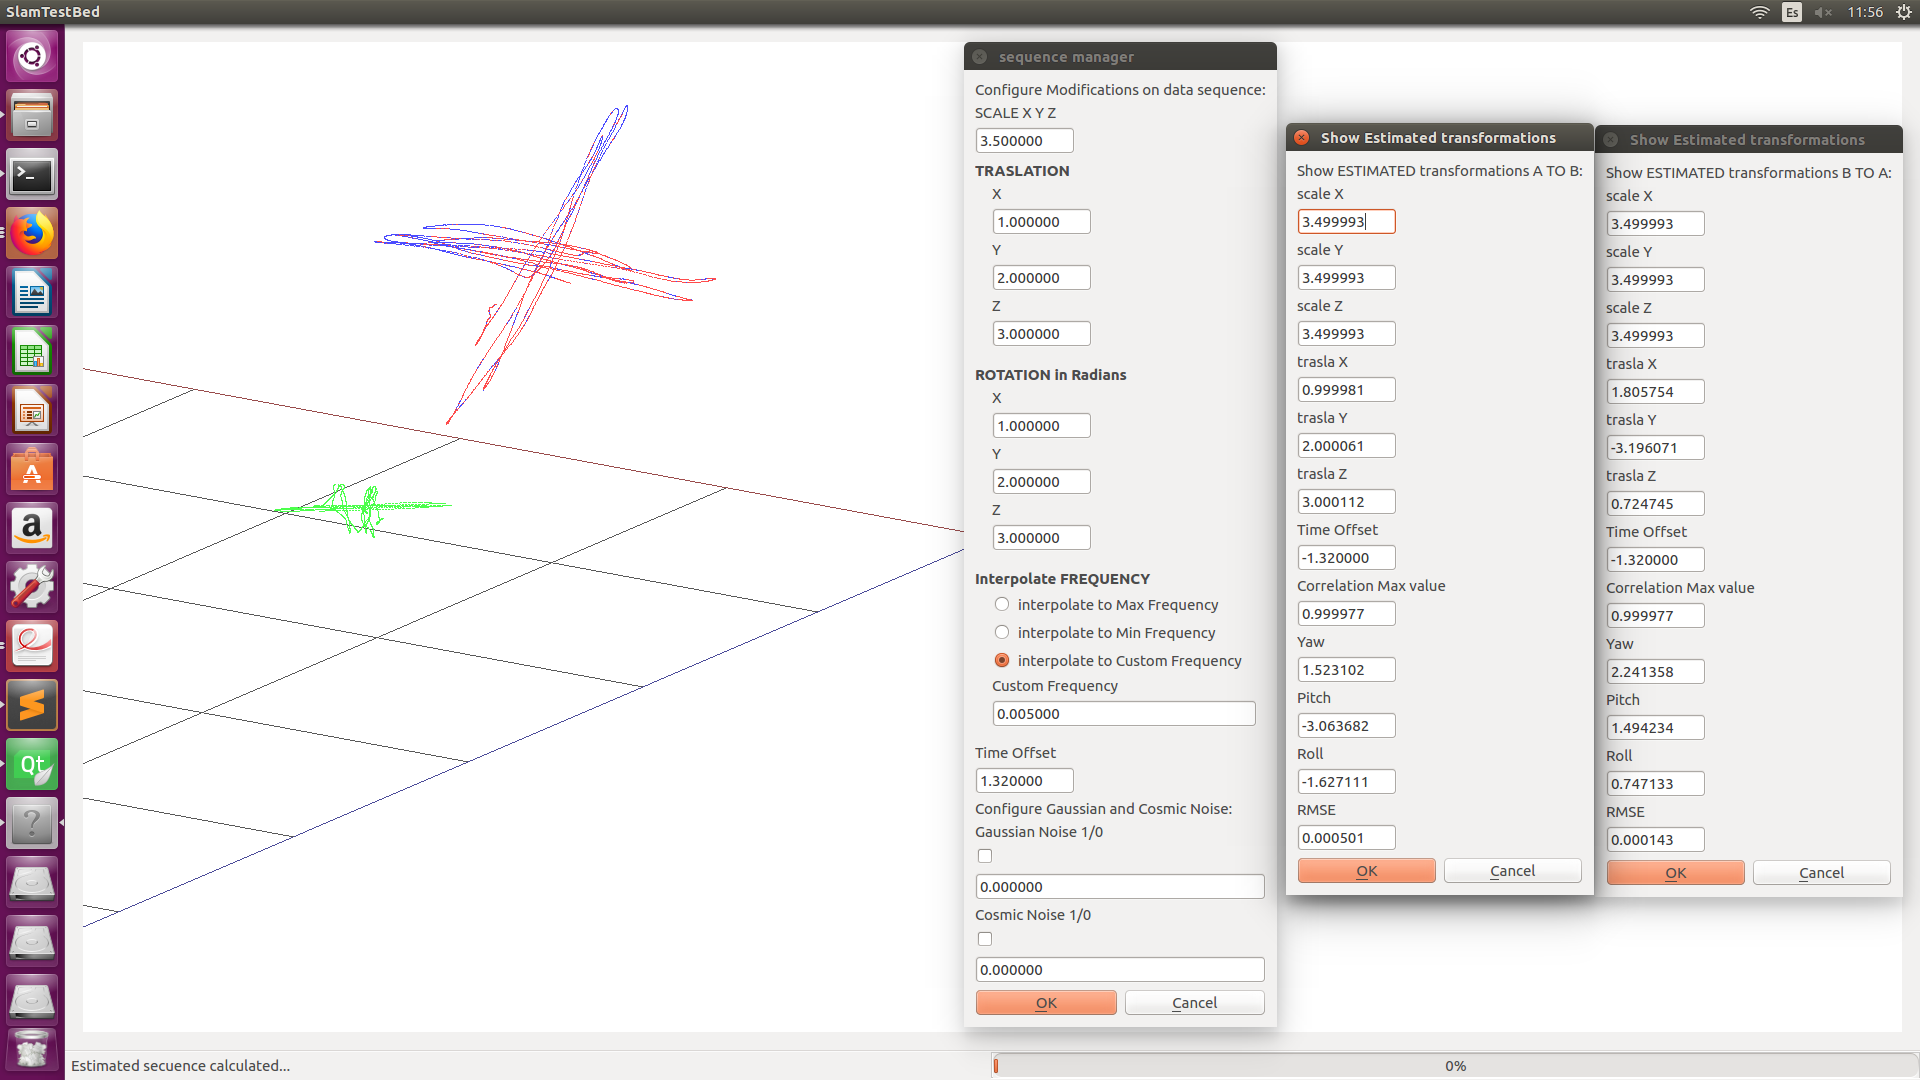
\includegraphics[height=10.0cm,width=15.0cm]{img/cap6/Escala_Trasla_Rota_Offset_abba.png}}
\hspace{0.5cm}

\end{center}

\caption{Gráfico que muestra los resultados de la estimación de un cambio de escala, traslación,rotación y offset .}
\end{figure}

Arriba en la imagen , se presenta el dataset original en verde, el dataset transformado en azul y el dataset estimado en rojo.
En este caso se ha realizado la siguiente combinación de transformaciónes, Escala, Traslación, Rotación y Offset.
Como se puede observar en los resultados de las estimaciones, el offset es estimado con total exactitud. Sin embargo el valor del RMSE ya no es de 0.0, si no de 0.0005, aún así el error cometido sigue siendo muy bajo.
Visualmente, también se puede observar que la precisión ha disminiuido , ya que se aprecian más puntos rojos (dataset estimado) en el gráfico. Esto indica que la estimación sigue siendo muy buena aunque la precisión ha bajado.


\begin{figure}[H]
\begin{center}
\subfigure[]{\label{fig:opciones de View}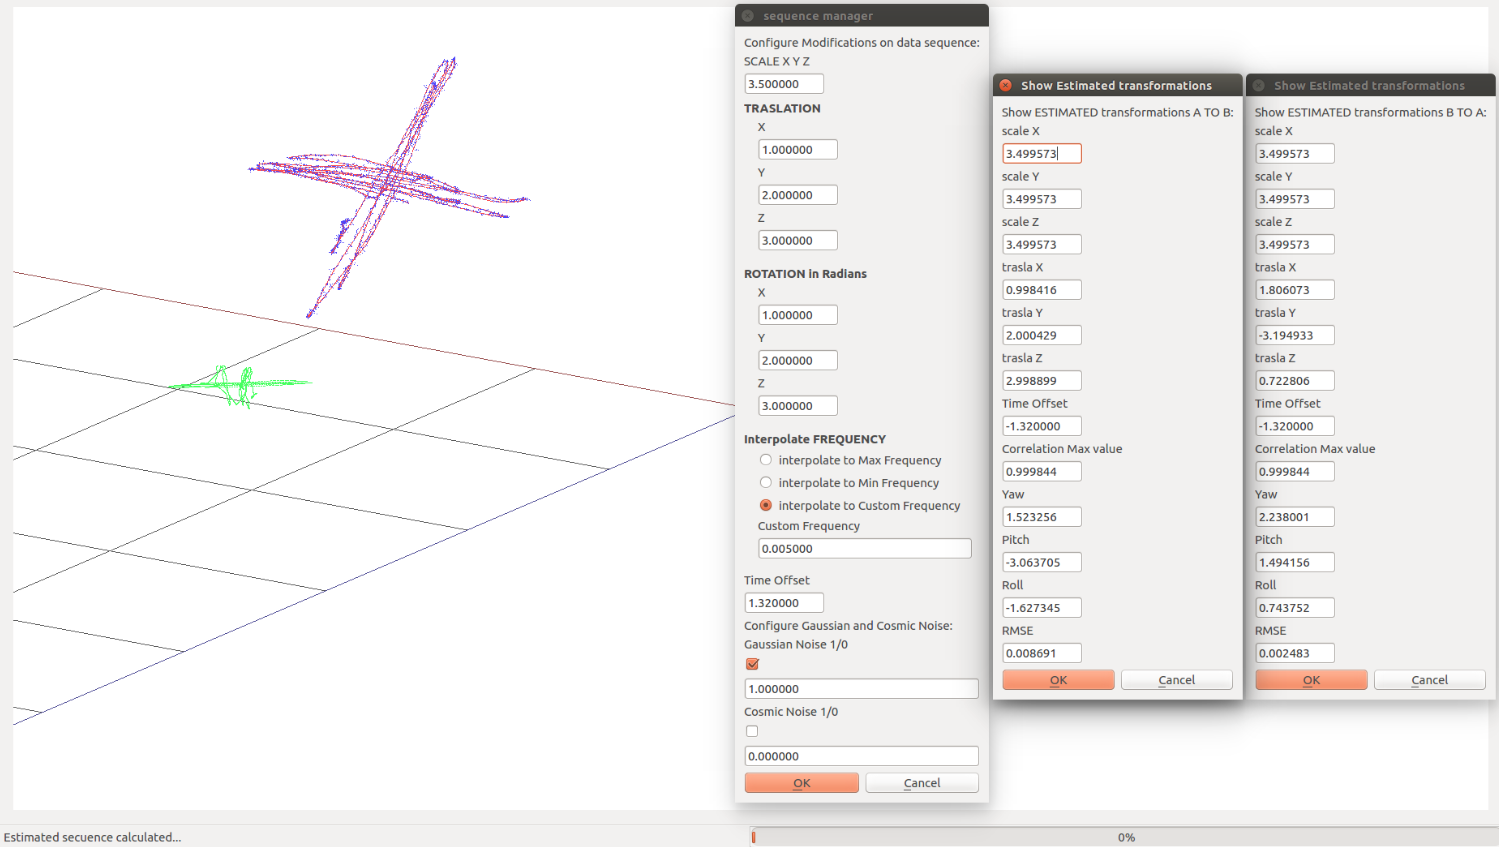
\includegraphics[height=10.0cm,width=15.0cm]{img/cap6/Escala_Trasla_Rota_Offset_GaussNoise_abba.png}}
\hspace{0.5cm}

\end{center}

\caption{Gráfico que muestra los resultados de la estimación de un cambio de escala y traslación .}
\end{figure}

En la imagen superior, podemos ver el dataset original en verde, el dataset transformado en azul y el dataset estimado en rojo.
Las transformaciones realizadas en este caso han sido, Escala, Traslación, Rotación, Offset y Ruido Gaussiano.
En este caso, al incluir ruido Gaussiano en la transformación del dataset original, el dataset estimado pierde precisión, y el RMSE obtenido es de  0.008.
Sin embargo, la precisión aunque es menor, continúa siendo buena, y en el gráfico puede verse , como el dataset estimado concuerda de manera aceptable con el dataset estimado.
Observesé que en el dataset estimado no hay ruido gaussiano.


\begin{figure}[H]
\begin{center}
\subfigure[]{\label{fig:opciones de View}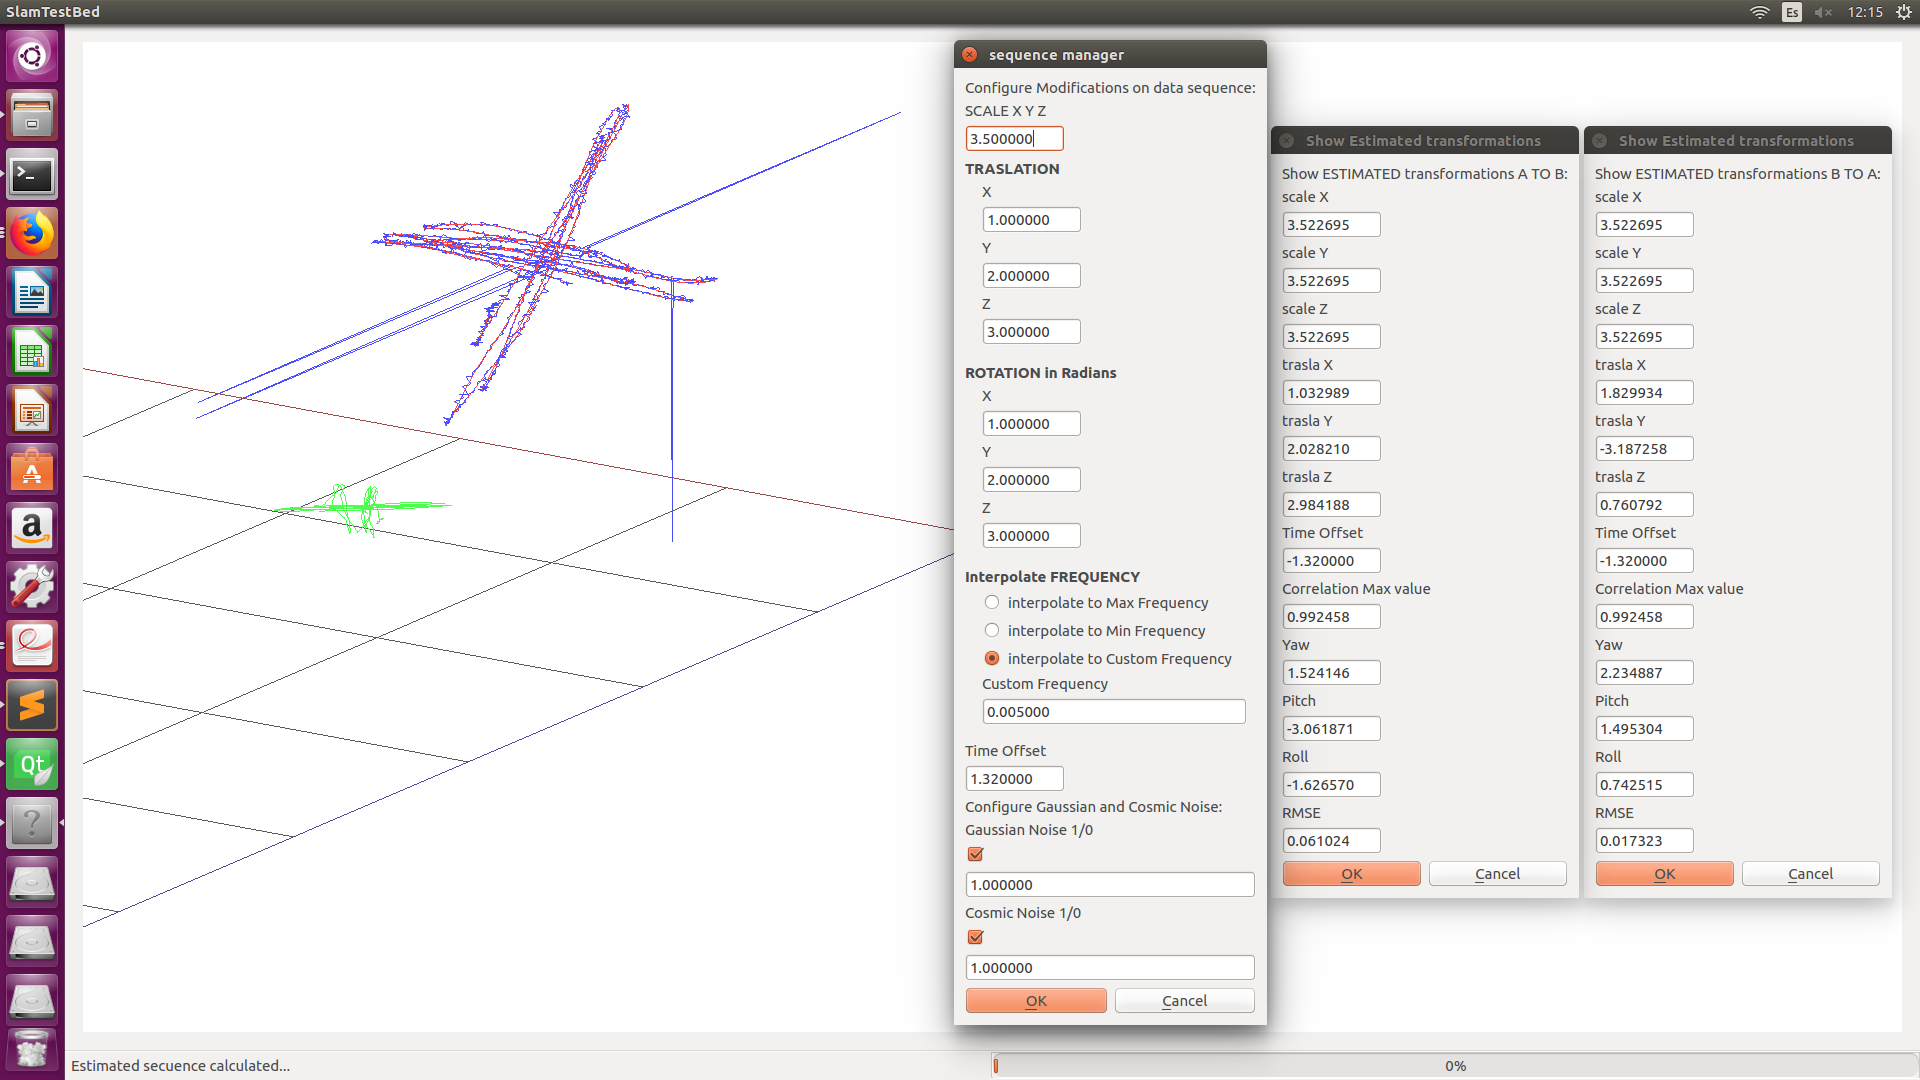
\includegraphics[height=10.0cm,width=15.0cm]{img/cap6/Escala_Trasla_Rota_Offset_Gauss_CosmicNoise_abba.png}}
\hspace{0.5cm}

\end{center}

\caption{Gráfico que muestra los resultados de la estimación de un cambio de escala y traslación .}
\end{figure}

Arriba podemos ver una nueva captura de pantalla, donde se han realizado las siguientes transformaciones, Escala, Traslación, Rotación, Offset, Ruido Gaussiano y Ruido Cósmico.
Como se puede observar, en las estimaciones del dataset A ( verde ) al dataset B (azul), la precisión ha bajado notablemente, con un valor RMSE del 0.06.
Esta precisión tan baja se debe a la incluisión de ruido Cósmico, que altera notablemente los valores de X, Y , Z  de algunos puntos 3D.
Aún así, como puede verse en  la representación gráfica del dataset Estimado (rojo) sobre el dataset Transformado ( azul ) se aproxima bastante a la solución óptima.



\begin{figure}[H]
\begin{center}
\subfigure[]{\label{fig:opciones de View}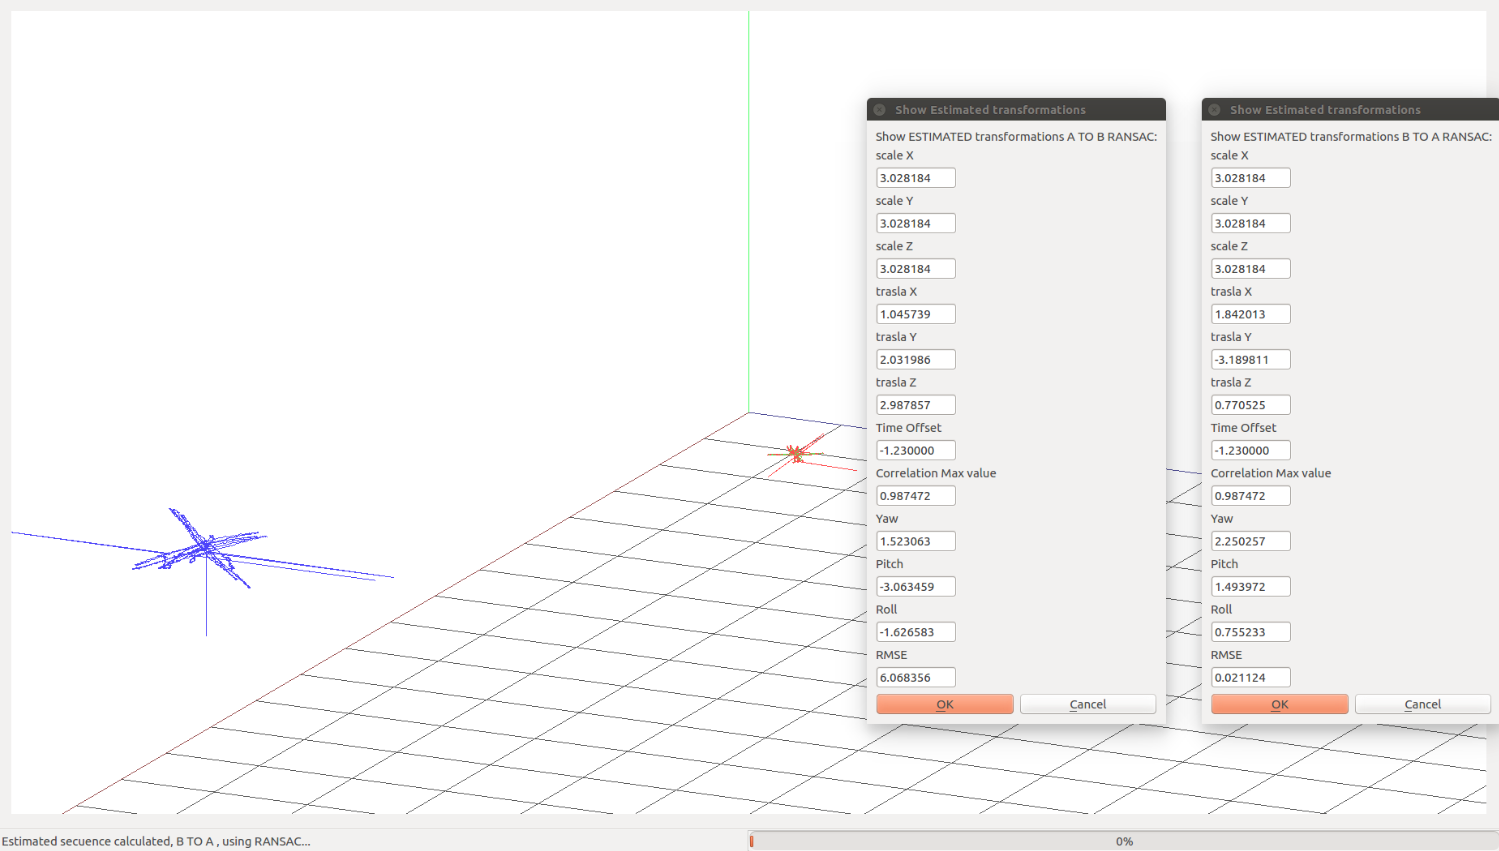
\includegraphics[height=8.0cm,width=12.0cm]{img/cap6/LoadTwoDataSets_RANSAC.png}}
\hspace{0.5cm}

\end{center}

\caption{Gráfico que muestra los resultados de la estimación de la transformación del datasetA en el datasetB y viceversa, utilizando RANSAC.}
\end{figure}

En captura de pantalla superior, podremos ver una nueva transformación donde se ha aplicado transformaciónes de Escala, Traslación, Rotación, Offset, Ruido Gaussiano y Cósmico y además se ha utilizado el método RANSAC para calcular el error.

\clearpage





%\begin{figure}[H]
%\begin{center}
%\subfigure[]{\label{fig:opciones de View}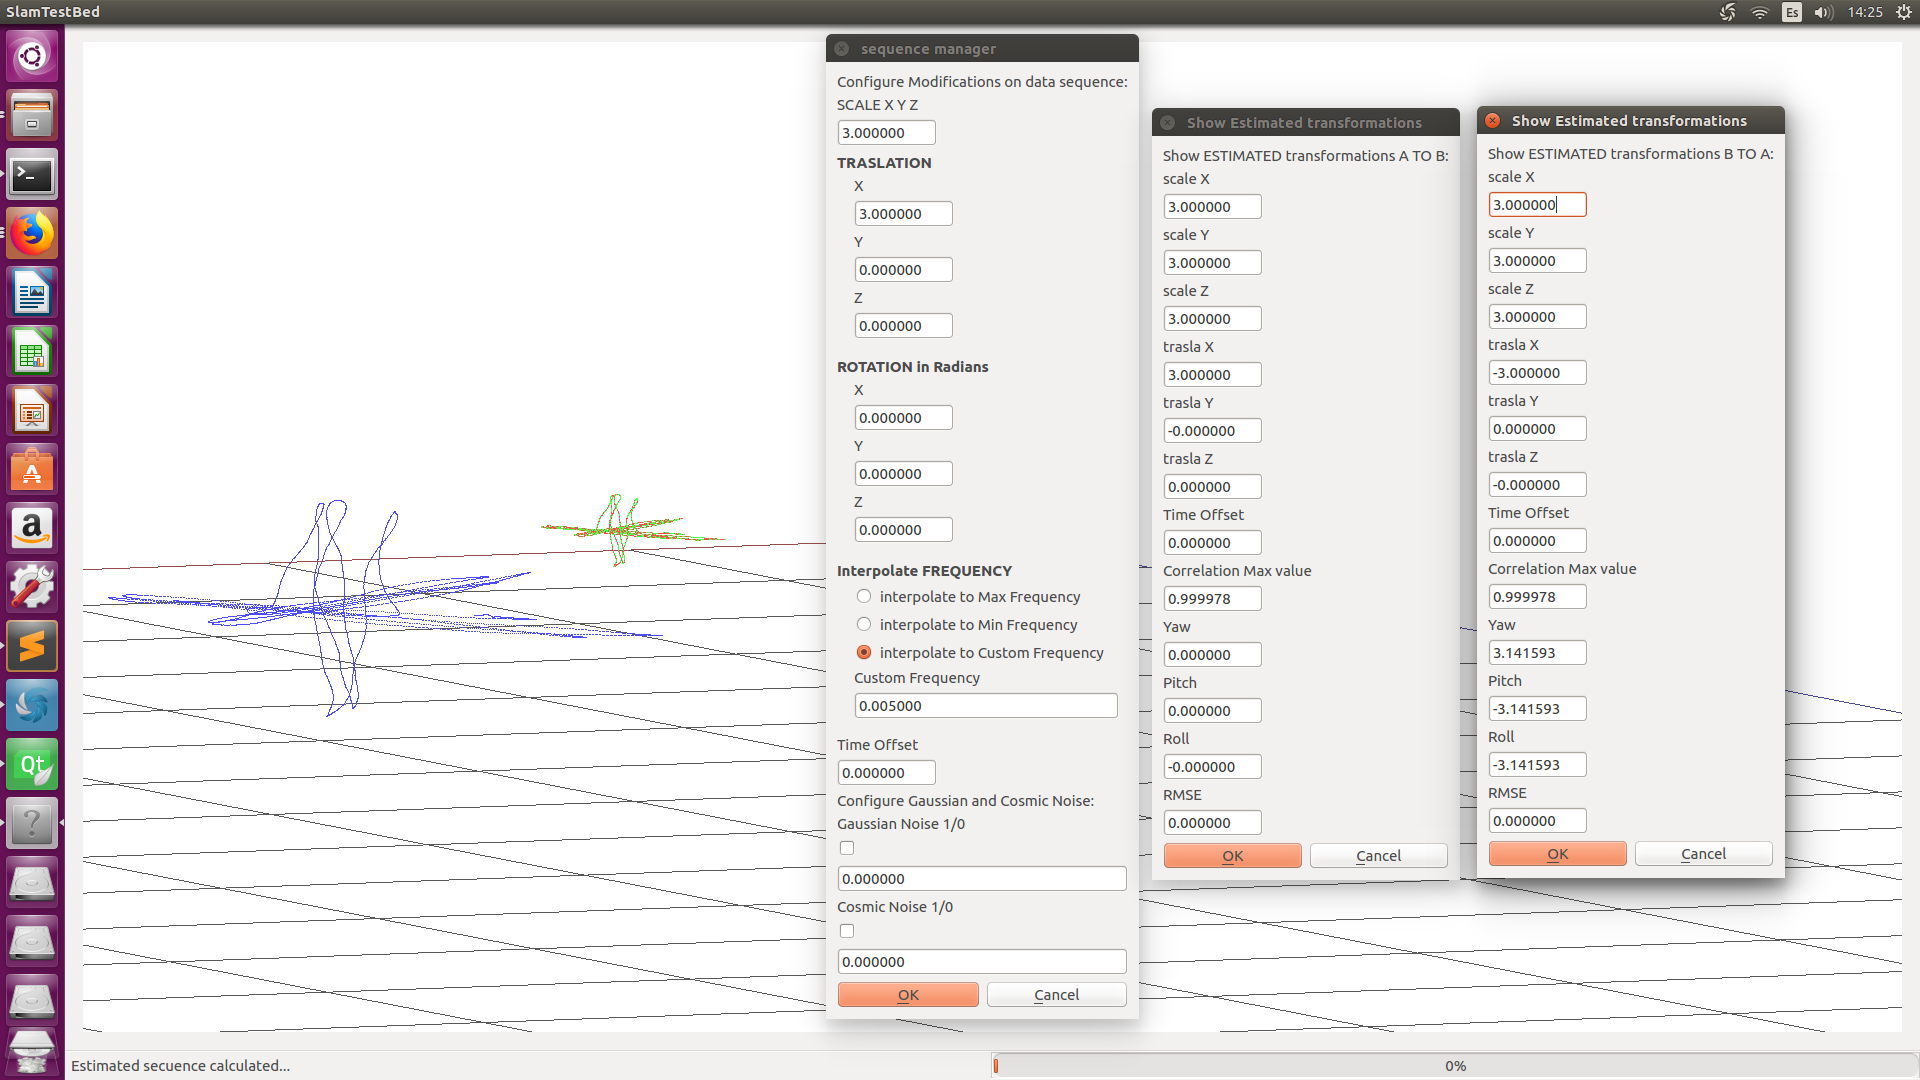
\includegraphics[height=8.0cm,width=12.0cm]{img/cap6/ScaleTraslaFrec.png}}
%\hspace{0.5cm}

%\end{center}

%\caption{Gráfico que muestra los resultados de la estimación de un cambio de escala, traslación y frecuencia.}
%\end{figure}


%\begin{figure}[H]
%\begin{center}
%\subfigure[]{\label{fig:opciones de View}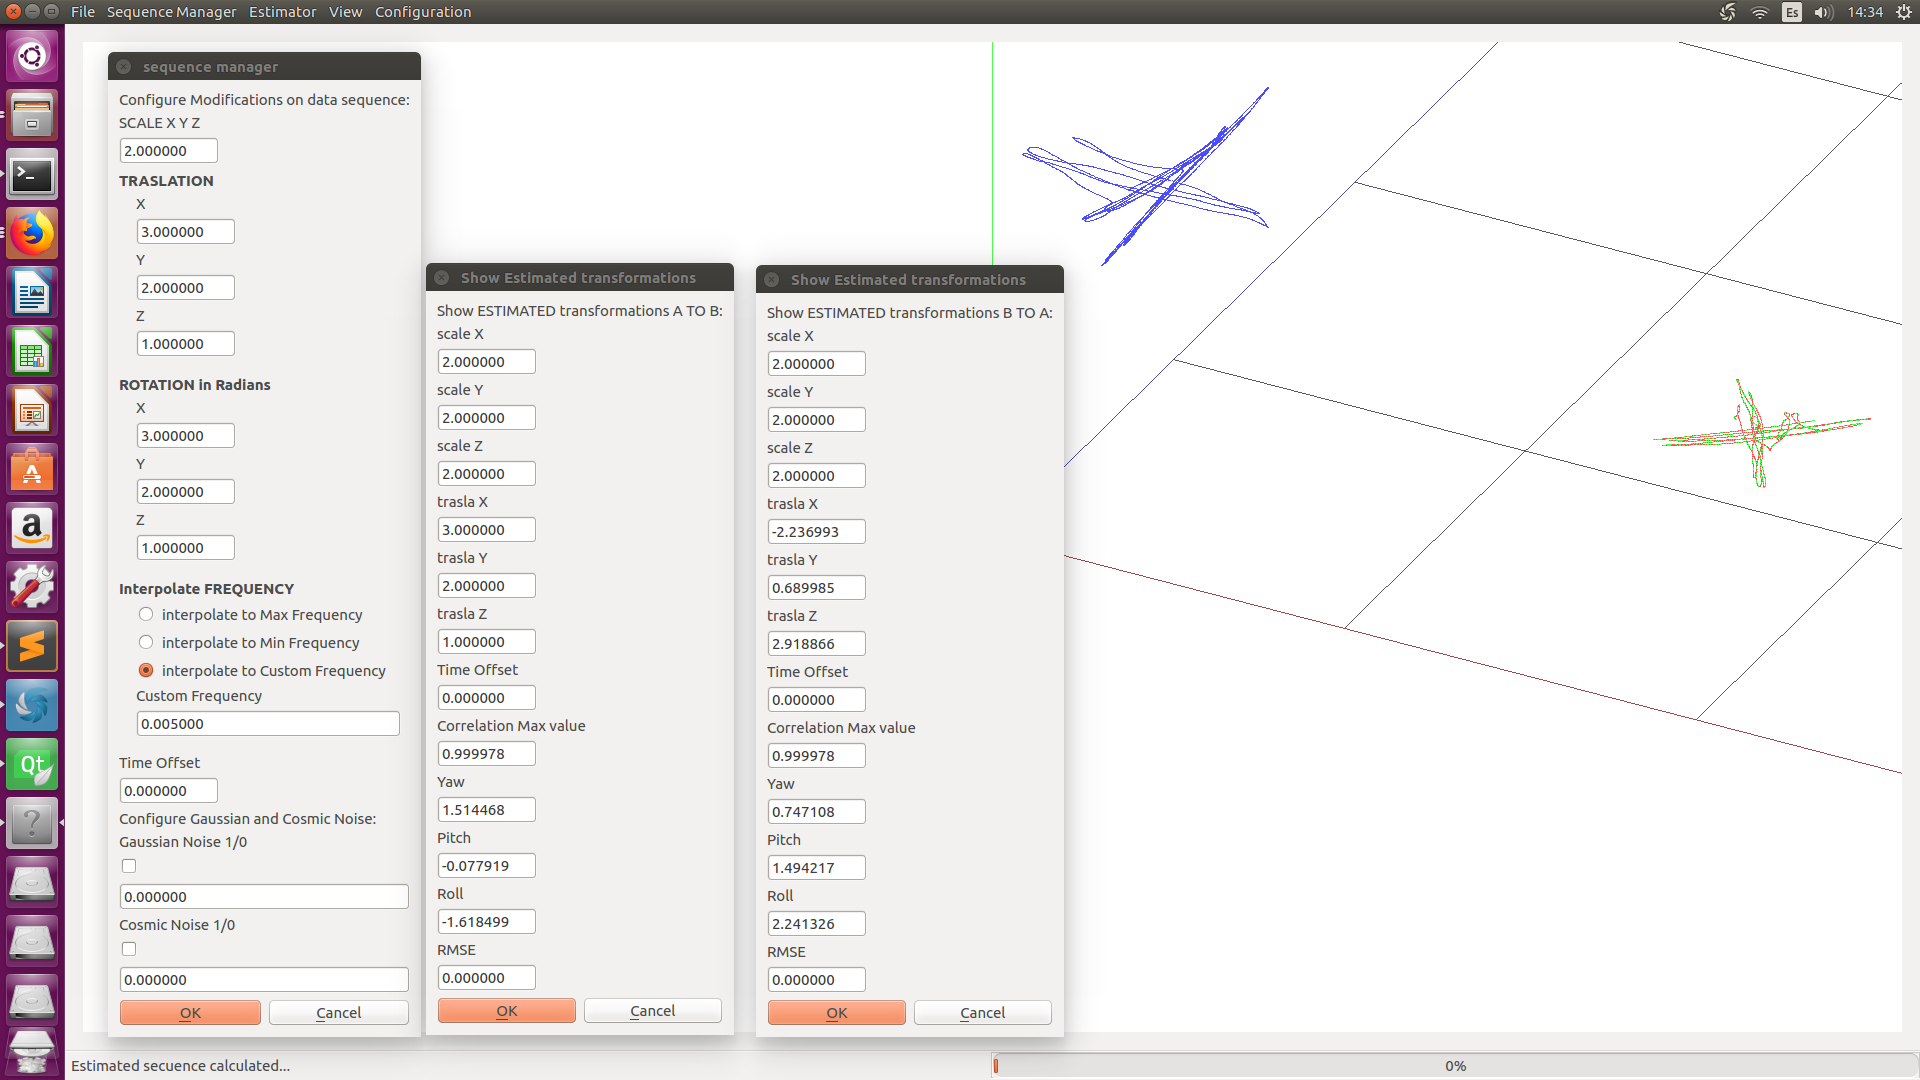
\includegraphics[height=8.0cm,width=12.0cm]{img/cap6/ScaleTraslaRotaFrec.png}}
%\hspace{0.5cm}

%\end{center}

%\caption{Gráfico que muestra los resultados de la estimación de un cambio de escala, traslación,rotación y frecuencia.}
%\end{figure}


%\begin{figure}[H]
%\begin{center}
%\subfigure[]{\label{fig:opciones de View}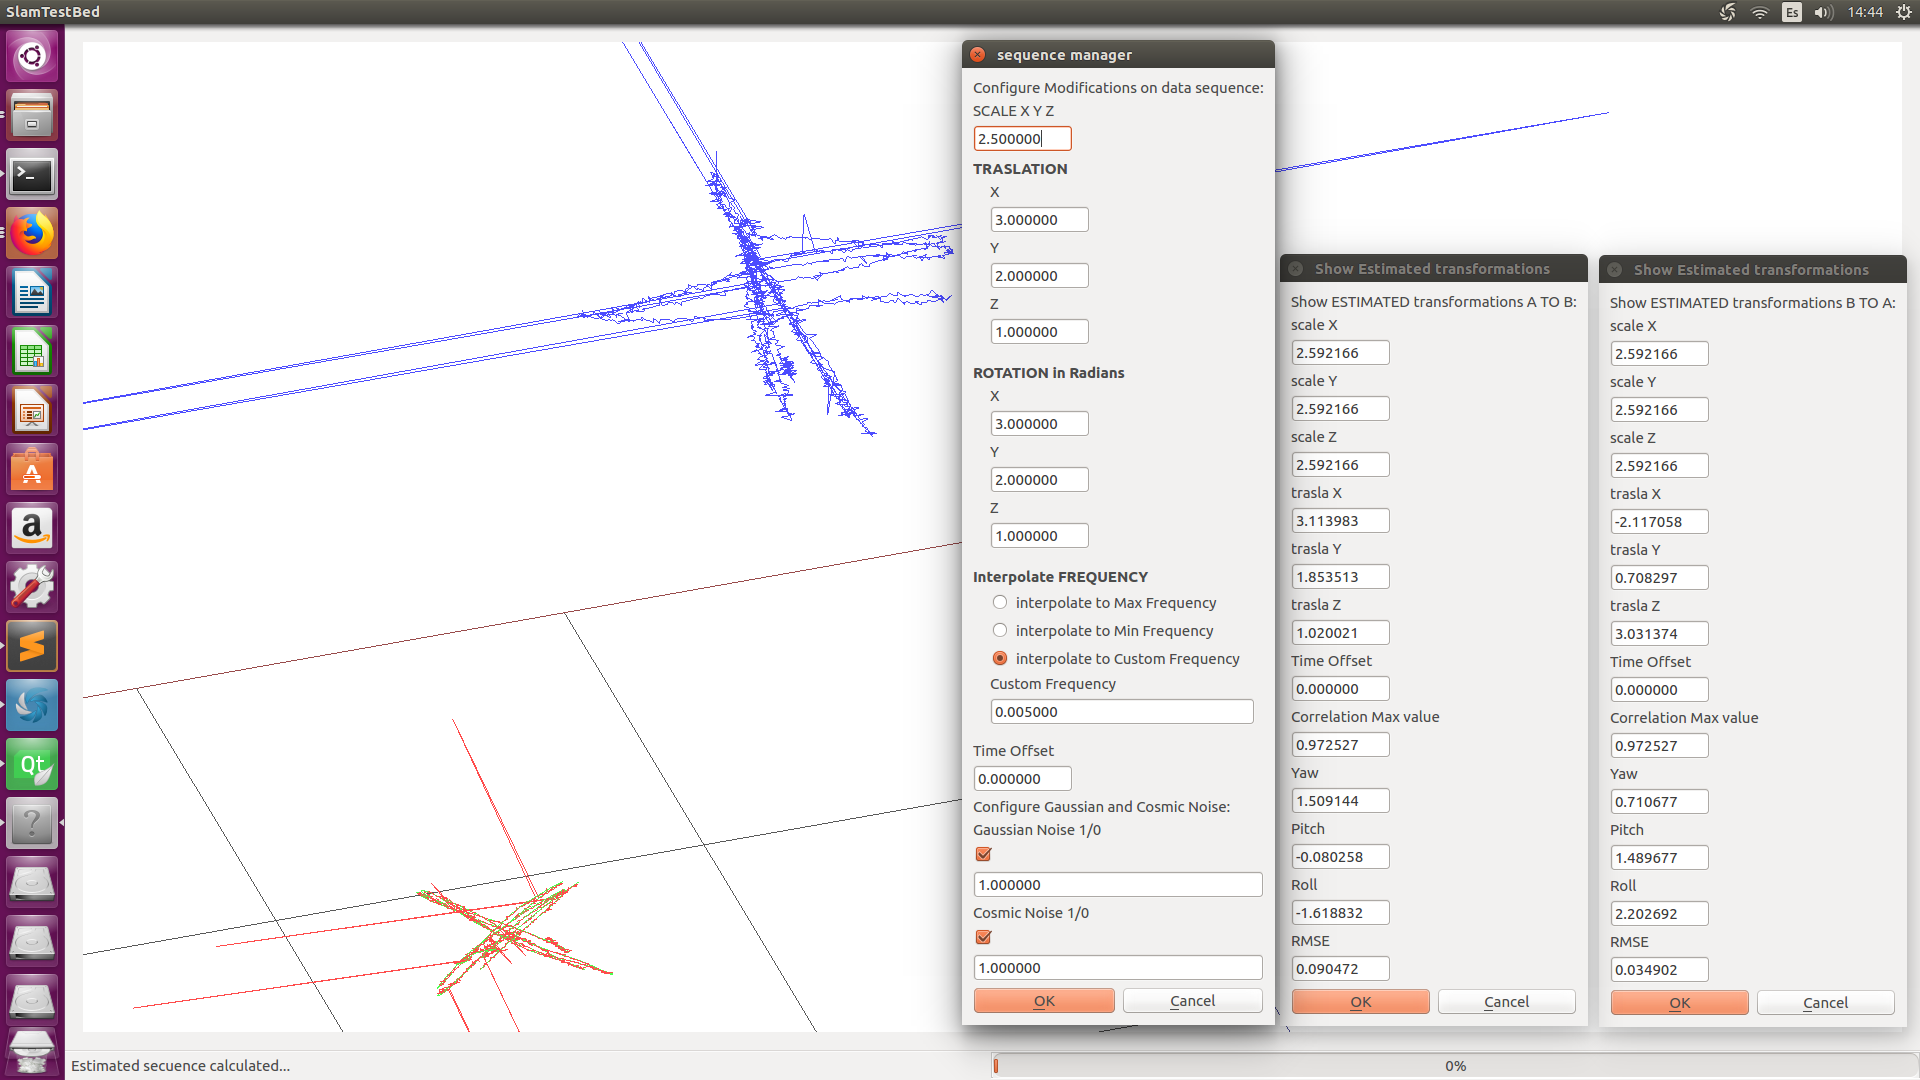
\includegraphics[height=8.0cm,width=12.0cm]{img/cap6/ScaleTraslaRotaFrecGNoiseCNoise.png}}
%\hspace{0.5cm}

%\end{center}

%\caption{Gráfico que muestra los resultados de la estimación de un cambio de escala, traslación, rotación, frecuencia, ruido gaussiano y ruido cósmico.}
%\end{figure}



%\begin{figure}[H]
%\begin{center}
%\subfigure[]{\label{fig:opciones de View}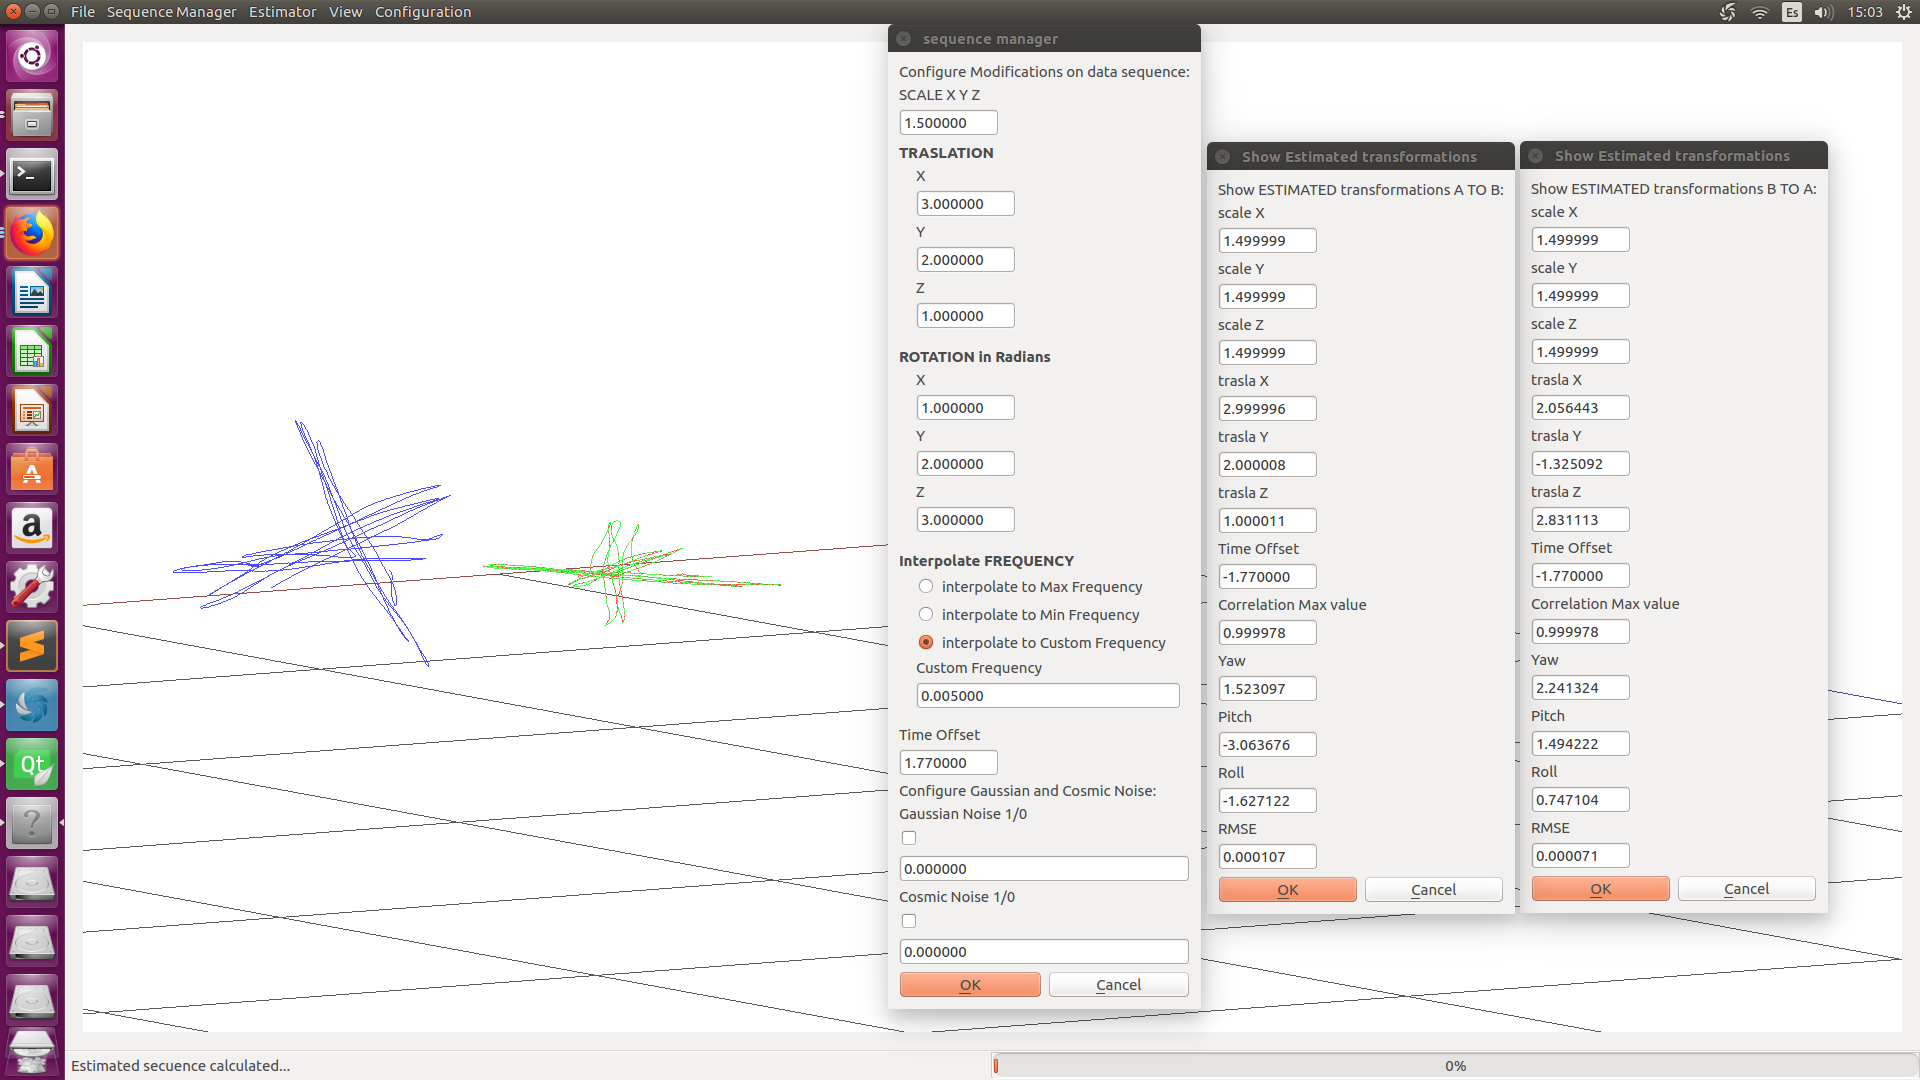
\includegraphics[height=8.0cm,width=12.0cm]{img/cap6/ScaleTraslaRotaFrecTimeOffset.png}}
%\hspace{0.5cm}

%\end{center}

%\caption{Gráfico que muestra los resultados de la estimación de un cambio de escala, traslación, rotación, frecuencia y offset.}
%\end{figure}


%\begin{figure}[H]
%\begin{center}
%\subfigure[]{\label{fig:opciones de View}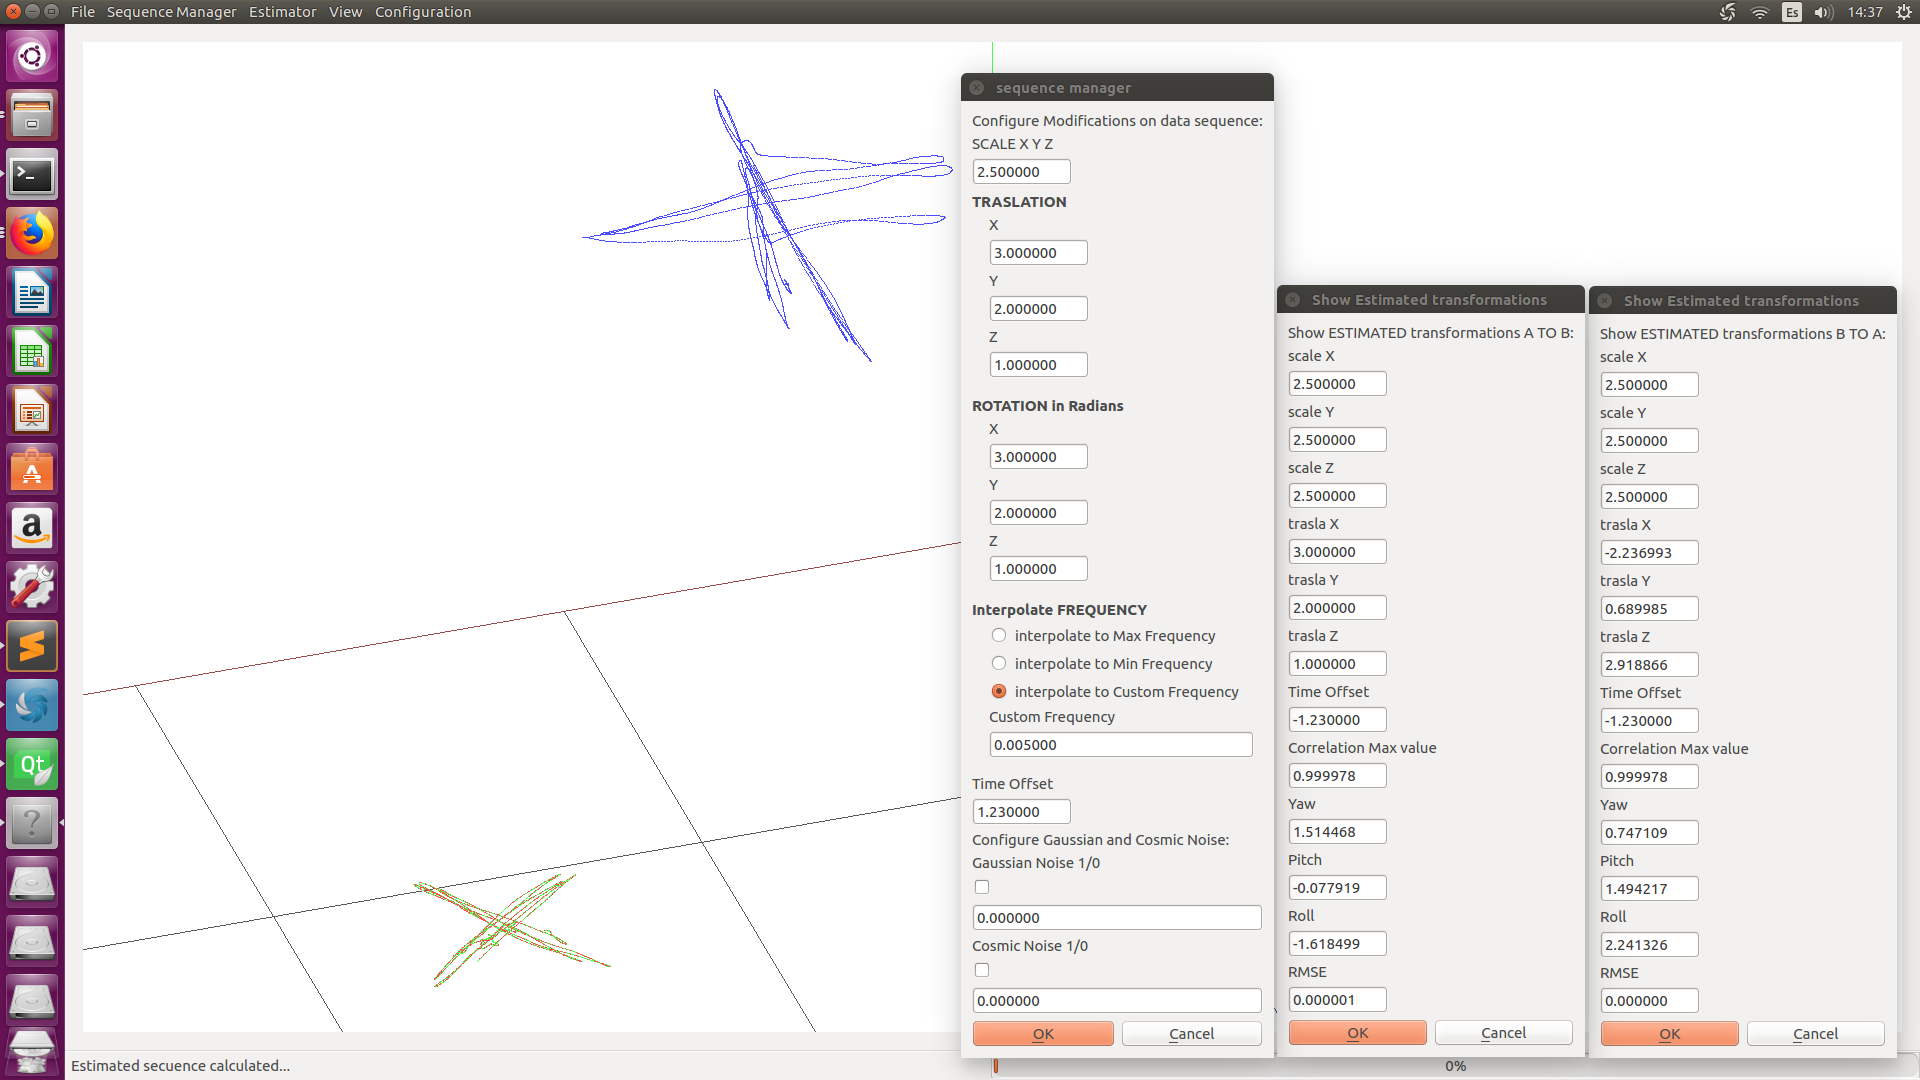
\includegraphics[height=8.0cm,width=12.0cm]{img/cap6/ScaleTraslaRotaFrecTimeOffset2.png}}
%\hspace{0.5cm}

%\end{center}

%\caption{Gráfico que muestra los resultados de la estimación de un cambio de escala, traslación, rotación, frecuencia y offset.}
%\end{figure}



%\begin{figure}[H]
%\begin{center}
%\subfigure[]{\label{fig:opciones de View}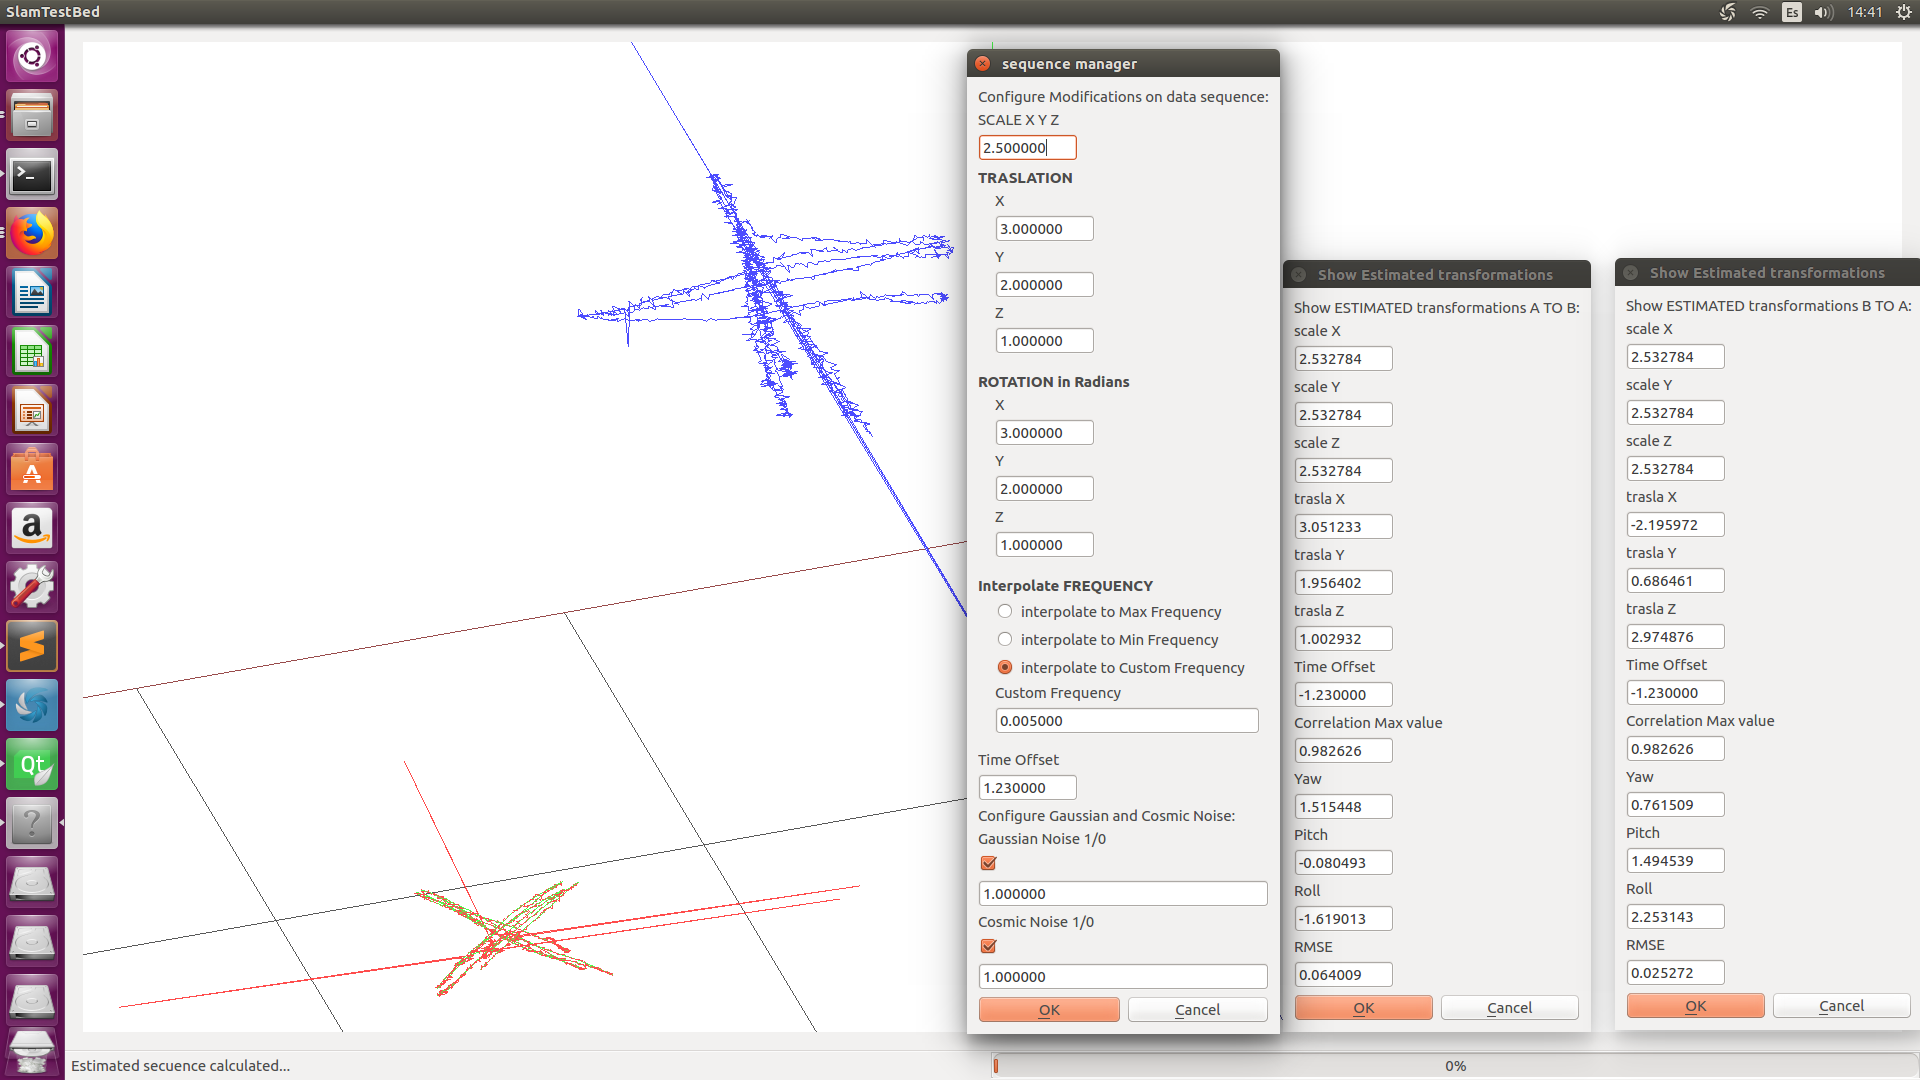
\includegraphics[height=8.0cm,width=12.0cm]{img/cap6/ScaleTraslaRotaFrecTimeOffsetGNoiseCNoise.png}}
%\hspace{0.5cm}

%\end{center}

%\caption{Gráfico que muestra los resultados de la estimación de un cambio de escala, traslación, rotación, frecuencia, Offset, Ruido Gausiano y Ruido Cósmico.}
%\end{figure}




%\begin{figure}[H]
%\begin{center}
%\subfigure[]{\label{fig:opciones de View}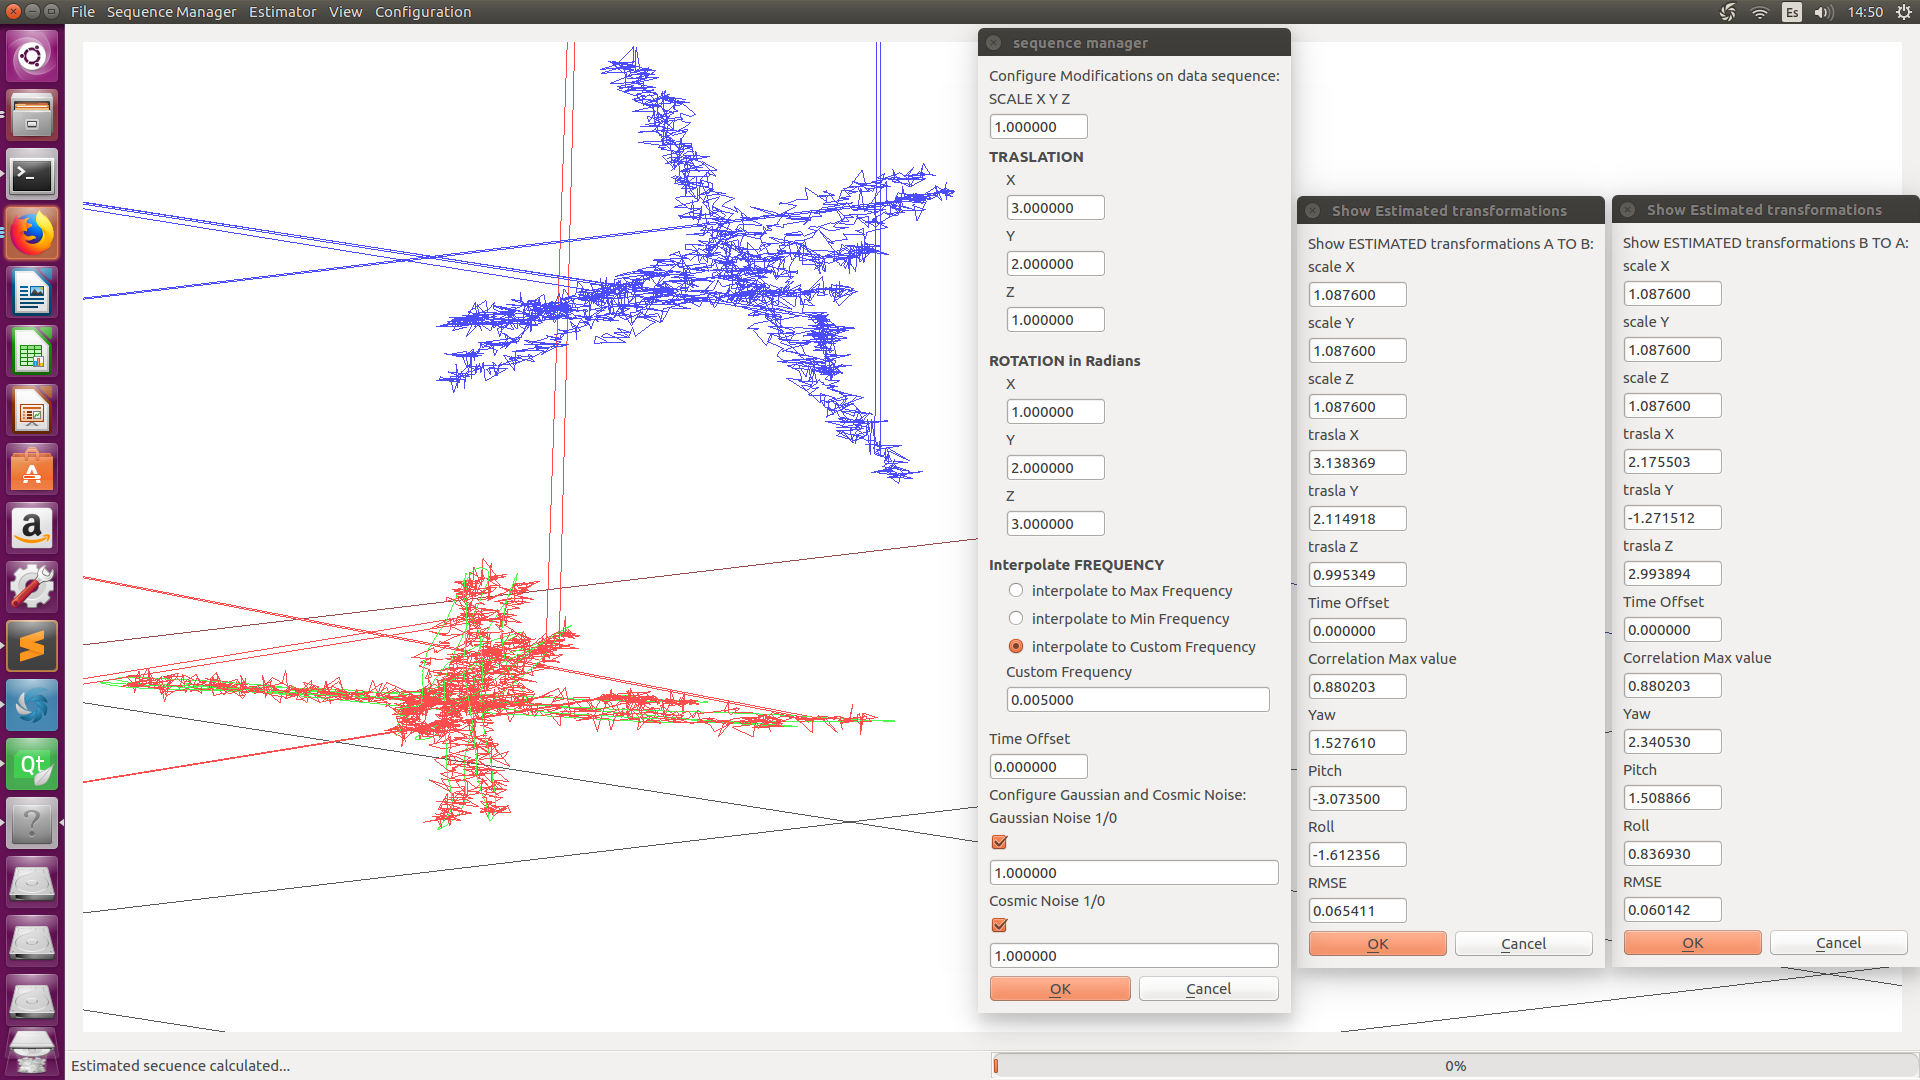
\includegraphics[height=8.0cm,width=12.0cm]{img/cap6/TraslaRotaFrecGnoiseCnoise.png}}
%\hspace{0.5cm}

%\end{center}

%\caption{Gráfico que muestra los resultados de la estimación de un cambio de traslación, rotación, frecuencia, Ruido Gaussiano y Ruido Cósmico.}
%\end{figure}


%Por último también mostraremos como SLAMTestBed es capaz de operar con 2 datasets diferentes , es decir en este caso , el seguno dataset no será el resultado de aplicar el módulo %de transformación sobre el primer dataset.

%\begin{figure}[H]
%\begin{center}
%\subfigure[]{\label{fig:opciones de View}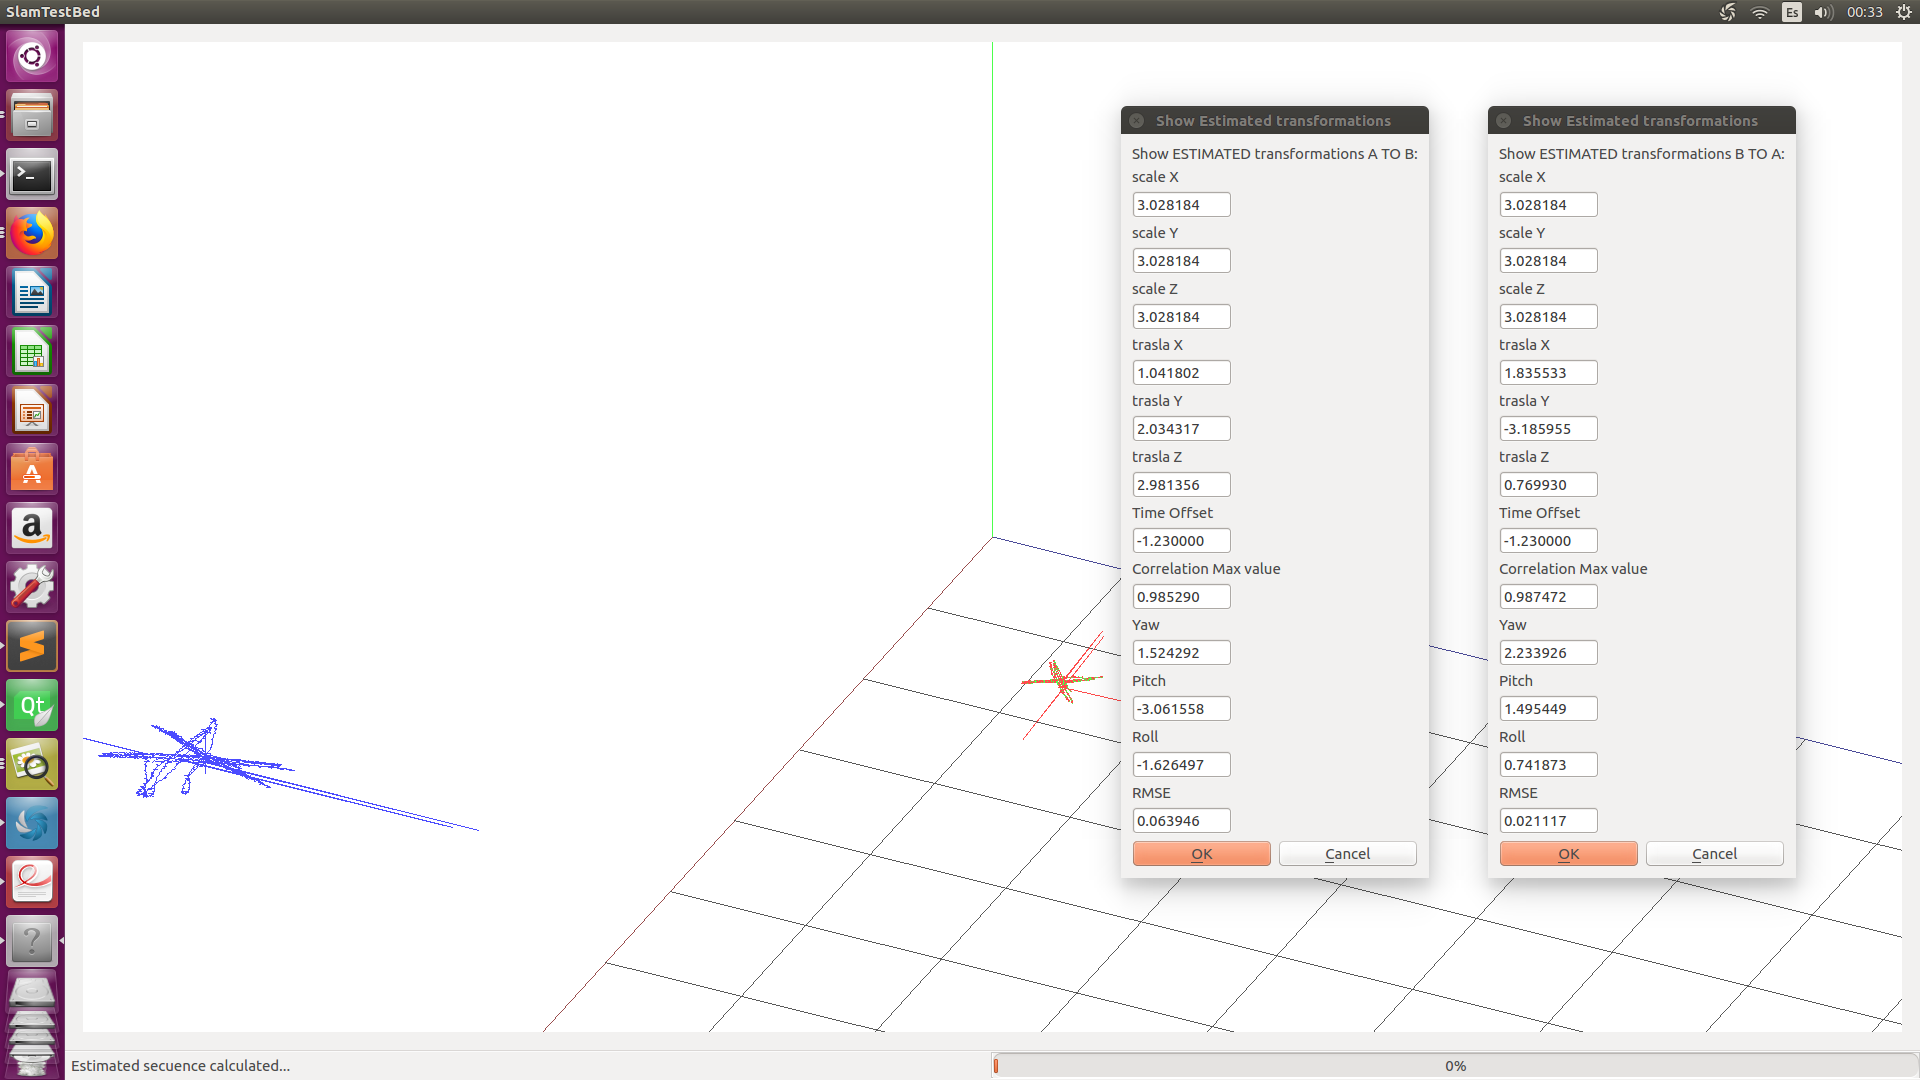
\includegraphics[height=8.0cm,width=12.0cm]{img/cap6/LoadTwoDataSets.png}}
%\hspace{0.5cm}

%\end{center}

%\caption{Gráfico que muestra los resultados de la estimación de la transformación del datasetA en el datasetB y viceversa.}
%\end{figure}


%\begin{figure}[H]
%\begin{center}
%\subfigure[]{\label{fig:opciones de View}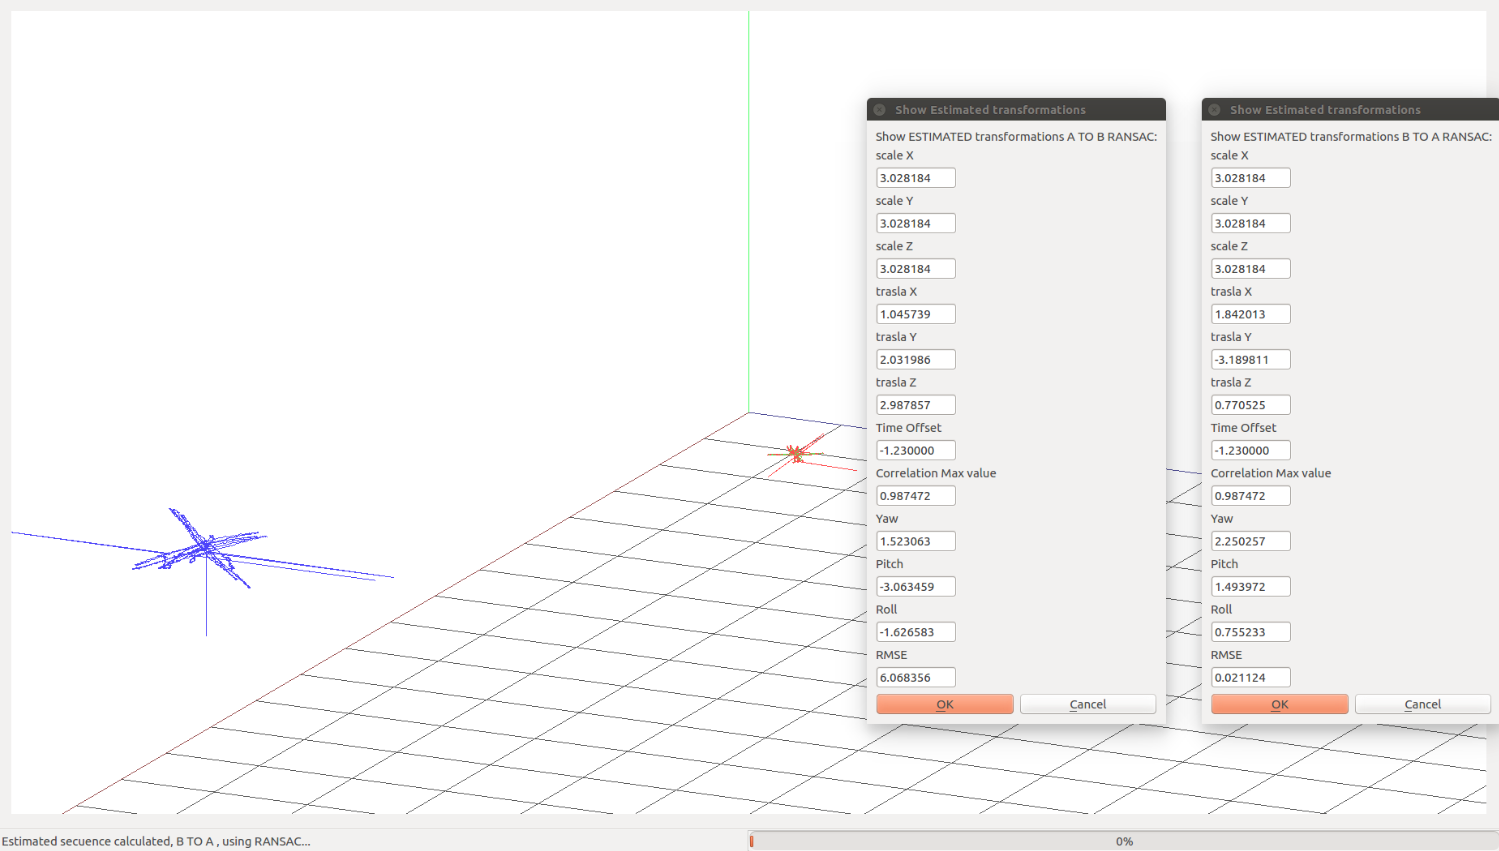
\includegraphics[height=8.0cm,width=12.0cm]{img/cap6/LoadTwoDataSets_RANSAC.png}}
%\hspace{0.5cm}

%\end{center}

%\caption{Gráfico que muestra los resultados de la estimación de la transformación del datasetA en el datasetB y viceversa, utilizando RANSAC.}
%\end{figure}

%\clearpage


